\documentclass[twocolumn, natbib]{svjour3}
%DIF LATEXDIFF DIFFERENCE FILE
%DIF DEL submission/report/report.tex   Fri Feb 13 15:20:06 2015
%DIF ADD revision/report/report.tex     Fri Mar 20 18:39:30 2015
\usepackage{graphicx}%GRaphiken
\usepackage[utf8]{inputenc}
\usepackage{tabularx}%Tabellen!
\usepackage[english]{babel}
\usepackage{textcomp}% Sonderzeichen
\usepackage{amsmath}%maths / equations
\usepackage{mathptmx}
\usepackage{url}
\usepackage{marvosym}
\newcommand{\envelope}{(\raisebox{-.5pt}{\scalebox{1.45}{\Letter}}\kern-.1pt) }

%DIF 13a13-22
% to compare to old %DIF > 
% cd /home/edisz/Documents/Uni/Projects/PHD/6USETHEGLM/manuscript/ %DIF > 
% % first compare bibliography %DIF > 
% latexdiff submission/report/report.bbl revision/report/report.bbl > revision/diff/diff.bbl %DIF > 
 %DIF > 
% % then document %DIF > 
% latexdiff --disable-citation-markup --math-markup=3 -t CTRADITIONAL submission/report/report.tex revision/report/report.tex > revision/diff/diff.tex %DIF > 
 %DIF > 
 %DIF > 
 %DIF > 
%DIF -------
%% ----------------------------------------------------------------------------
\title{Ecotoxicology is not normal.}
%DIF 15c25
%DIF < \subtitle{How the use of proper statistical models can increase statistical power in ecotoxicological experiments.}
%DIF -------
\subtitle{A comparison of statistical approaches for analysis of count and proportion data in ecotoxicology.} %DIF > 
%DIF -------
\author{Eduard Szöcs \and Ralf B. Schäfer}
\institute{Eduard Szöcs \envelope  and Ralf B. Schäfer \at
Institute for Environmental Sciences \\
University Koblenz-Landau \\
Fortstraße 7, \\
76829 Landau, Germany \\
Tel.: +49 06341 280 31552 \\
\email{szoecs@uni-landau.de}
}
\date{Received: date / Accepted: date}
\journalname{Environmental Science and Pollution Research}



%% ----------------------------------------------------------------------------
%DIF PREAMBLE EXTENSION ADDED BY LATEXDIFF
%DIF UNDERLINE PREAMBLE %DIF PREAMBLE
\RequirePackage[normalem]{ulem} %DIF PREAMBLE
\RequirePackage{color}\definecolor{RED}{rgb}{1,0,0}\definecolor{BLUE}{rgb}{0,0,1} %DIF PREAMBLE
\providecommand{\DIFadd}[1]{{\protect\color{blue}\uwave{#1}}} %DIF PREAMBLE
\providecommand{\DIFdel}[1]{{\protect\color{red}\sout{#1}}}                      %DIF PREAMBLE
%DIF SAFE PREAMBLE %DIF PREAMBLE
\providecommand{\DIFaddbegin}{} %DIF PREAMBLE
\providecommand{\DIFaddend}{} %DIF PREAMBLE
\providecommand{\DIFdelbegin}{} %DIF PREAMBLE
\providecommand{\DIFdelend}{} %DIF PREAMBLE
%DIF FLOATSAFE PREAMBLE %DIF PREAMBLE
\providecommand{\DIFaddFL}[1]{\DIFadd{#1}} %DIF PREAMBLE
\providecommand{\DIFdelFL}[1]{\DIFdel{#1}} %DIF PREAMBLE
\providecommand{\DIFaddbeginFL}{} %DIF PREAMBLE
\providecommand{\DIFaddendFL}{} %DIF PREAMBLE
\providecommand{\DIFdelbeginFL}{} %DIF PREAMBLE
\providecommand{\DIFdelendFL}{} %DIF PREAMBLE
%DIF END PREAMBLE EXTENSION ADDED BY LATEXDIFF

\begin{document}
\DIFaddbegin \sloppy
\DIFaddend \maketitle

%% ----------------------------------------------------------------------------
\begin{abstract}
\DIFdelbegin \DIFdel{Ecotoxicologists are often confronted with non-normally distributed data .
}\DIFdelend \DIFaddbegin \DIFadd{Counts and proportions are data types of encountered by ecotoxicologists.
However, such data is rare normally distributed.
}\DIFaddend To meet the assumptions of normality and heteroscedasticity, the standard procedure has been to either transform the data or use non-parametric methods if this fails.
\DIFaddbegin \DIFadd{Generalised Linear Models (GLM) allow to model directly distributions fitting to such data.
}\DIFaddend Here, we compare the \DIFdelbegin \DIFdel{statistical power of analyses using transformed dataor non-parametric methods to analyses using appropriate distributional assumptions, }%DIFDELCMD < \allowbreak %%%
\DIFdel{namely Generalised Linear Models (GLM) }\DIFdelend \DIFaddbegin \DIFadd{performance of methods assuming normality of transformed data, methods assuming appropriate distributions (Poisson, negativ binomial, binomial) and non-parametric methods}\DIFaddend .

We simulated data mimicking \DIFaddbegin \DIFadd{low replicated }\DIFaddend ecotoxicological experiments of two common data types (counts and proportions \DIFaddbegin \DIFadd{from counts}\DIFaddend ). 
We \DIFdelbegin \DIFdel{compare }\DIFdelend \DIFaddbegin \DIFadd{compared }\DIFaddend the performance of \DIFaddbegin \DIFadd{different }\DIFaddend methods in terms of statistical power and type 1 error \DIFaddbegin \DIFadd{for detecting a general treatment effect and determining the lowest observed effect concentration (LOEC)}\DIFaddend .
In addition, we outlined differences and advantages of GLMs on a real world mesocosm data set.

\DIFdelbegin \DIFdel{We found that GLMs provide in most cases a gain in statistical power compared to analysis of transformed data or using }\DIFdelend \DIFaddbegin \DIFadd{For counts, we found that the quasi-Poisson model and the negative binomial model in combination with parametric boostrap had higher statistical power then data transformation.
For proportions GLMs performed better, except to determine LOEC at extremly low sample sizes.
The compared }\DIFaddend non-parametric methods \DIFdelbegin \DIFdel{.
}\DIFdelend \DIFaddbegin \DIFadd{had generally lower power.
}

\DIFaddend We recommend that \DIFdelbegin \DIFdel{non-normal data }\DIFdelend \DIFaddbegin \DIFadd{counts and proportions from counts }\DIFaddend should be analysed by \DIFdelbegin \DIFdel{GLMs and not by transformations or non-parametric methods.
}\DIFdelend \DIFaddbegin \DIFadd{making appropriate distributional assumptions and }\DIFaddend GLMs should become a standard method in ecotoxicology.
 \keywords{Generalized Linear Models \and Transformations \and Simulation \and Power \and Type 1 error}
\end{abstract}




%% ----------------------------------------------------------------------------
\section{Introduction}
\label{sec:intro}
Ecotoxicologists perform various kinds of experiments yielding different types of data.
Examples are \DIFdelbegin \DIFdel{: }\DIFdelend animal counts in mesocosm experiments (\DIFdelbegin \DIFdel{positive}\DIFdelend \DIFaddbegin \DIFadd{non-negative}\DIFaddend , integer-valued data) \DIFdelbegin \DIFdel{, }\DIFdelend \DIFaddbegin \DIFadd{or }\DIFaddend proportions of surviving animals (data \DIFdelbegin \DIFdel{bonded }\DIFdelend \DIFaddbegin \DIFadd{bounded }\DIFaddend between 0 and 1, \DIFdelbegin \DIFdel{continuous)or biomass in growth experiments (positive, continuous data)}\DIFdelend \DIFaddbegin \DIFadd{discrete)}\DIFaddend .
These data are typically not normally distributed. 
Nevertheless, they are usually analysed using methods assuming a normal distribution and variance homogeneity \citep{wang_making_2011}. 
To meet these assumptions, data are usually transformed.
For example, ecotoxicological textbooks \citep{newman_quantitative_2012} and guidelines \citep{epa_methods_2002,oecd_current_2006} advise that survival data can be transformed using an arcsine square root transformation. 
For count data from mesocosm experiments a log(Ay + C) transformation is usually applied, where the constants A and C are either chosen arbitrarily or following general recommendations. 
For example, \citet{van_den_brink_impact_2000} suggest to set the term Ay to be 2 for the lowest abundance value (y) greater than zero and C to 1. 
Moreover, other transformations like the square root or fourth root are commonly applied in community ecology.
Note that there has been little evaluation and advice for practitioners, which transformations to use.
If the transformed data still do not meet the assumptions (i.e. normality and variance homogeneity), non-parametric tests are usually applied \citep{wang_making_2011}.

Generalised linear models (GLM) provide a method to analyse \DIFdelbegin \DIFdel{such non-normally distributed data }\DIFdelend \DIFaddbegin \DIFadd{counts or proportions from counts in a  statistically sound way }\DIFaddend \citep{nelder_generalized_1972}.
GLMs can handle various types of data distributions, e.g. Poisson or negative binomial (for count data) or binomial (for proportions); the normal distribution being a special case of GLMs.
Despite GLMs being available more than 40 years, ecotoxicologists do not regularly make use of them.
Recent studies concluded that data transformations should be avoided and GLMs be used as they have better statistical properties \DIFdelbegin %DIFDELCMD < \citep{ohara_not_2010, warton_arcsine_2011}%%%
\DIFdelend \DIFaddbegin \DIFadd{(}\citealt{ohara_not_2010} \DIFadd{(counts), }\citealt{warton_arcsine_2011,warton_many_2005} \DIFadd{(proportions from counts))}\DIFaddend . 

Ecotoxicological experiments often involve small sample sizes due to practical constraints. 
For example, extremely low samples sizes (n \textless 5) are common in many mesocosm studies \citep{sanderson_pesticide_2002,szocs_analysing_2015}.
Small sample sizes lead to low power in statistical hypothesis testing, on which many ecotoxiological approaches (e.g. risk assessment for pesticides) rely. 
Such an endpoint are L/NOEC (Lowest / No observed effect concentration) values.
Although their use has been heavily criticized in the past \citep{laskowski_good_1995}, they are \DIFdelbegin \DIFdel{still regularly used in ecotoxicology }%DIFDELCMD < \citep{jager_bad_2012}%%%
\DIFdel{.
Especially in mesocosm studies L/NOEC calculations are used in the majority of mesocosm }\DIFdelend \DIFaddbegin \DIFadd{the predominant endpoint in mesocosm }\DIFaddend experiments \citep{brock_minimum_2015, efsa_ppr_guidance_2013}. 

We explore how GLMs may enhance inference in ecotoxicological studies and compared three types of statistical methods (transformation and normality assumption, GLM, non-parametric tests).
We first illustrate differences between statistical methods using a data set from a mesocosm study.
Then we further elaborate differences in detecting a general treatment effect and determining the LOEC using simulations of two common data types in ecotoxicology: counts and proportions \DIFaddbegin \DIFadd{from counts}\DIFaddend . 



%% ----------------------------------------------------------------------------
\section{Methods}
\label{sec:methods}

%% --------------------------------
\subsection{Models for count data}
\DIFaddbegin \label{ssec:counts}
\DIFaddend \subsubsection{Linear model for transformed data}
To meet the assumptions of the standard linear model, count data usually needs to be transformed. 
We followed the recommendations of \citet{van_den_brink_impact_2000} and used a log(Ay + 1) transformation (eqn. \ref{eqn:trans}):
\DIFdelbegin %DIFDELCMD < 

%DIFDELCMD < %%%
\DIFdelend \begin{align}
  y\DIFdelbegin \DIFdel{^T_i}\DIFdelend \DIFaddbegin \DIFadd{_i^T }\DIFaddend & = log(Ay_i + 1) \label{eqn:trans}
\DIFdelbegin %DIFDELCMD < \\
%DIFDELCMD <   %%%
\DIFdel{A }%DIFDELCMD < & %%%
\DIFdel{= 2~/~min(y)~~~\text{, for}~ y > 0 }%DIFDELCMD < \nonumber
%DIFDELCMD < %%%
\DIFdelend \end{align}

, where $y_i$ is the measured \DIFdelbegin \DIFdel{abundance }\DIFdelend and $y_i^T$ the transformed abundance \DIFdelbegin \DIFdel{. 
}\DIFdelend \DIFaddbegin \DIFadd{of the $i$th observation. 
The factor $A$ was chosen in such way that $Ay$ equals 2 for the lowest non-zero abundance value (y).
}\DIFaddend 

Then we fitted the linear model to the transformed abundances (hereafter $LM$):
\DIFdelbegin %DIFDELCMD < 

%DIFDELCMD < %%%
\DIFdelend \begin{align}
  y_i^T &\sim N(\mu_i, \sigma^2) \nonumber \\
  \DIFaddbegin \DIFadd{E(}\DIFaddend y_i^T\DIFdelbegin %DIFDELCMD < &%%%
\DIFdelend \DIFaddbegin \DIFadd{) }\DIFaddend = \DIFdelbegin \DIFdel{\alpha + \beta x_i }%DIFDELCMD < \label{eqn:normal} \\
%DIFDELCMD <   %%%
\DIFdelend \DIFaddbegin \DIFadd{\mu_i ~}&\DIFadd{\text{and}~ }\DIFaddend var(y_i^T) \DIFdelbegin %DIFDELCMD < &%%%
\DIFdelend = \sigma^2 \DIFaddbegin \label{eqn:normal} \\
  \DIFadd{\mu_i }&\DIFadd{= \beta Treatment_i  }\DIFaddend \nonumber
\end{align}

This model assumes a normal distributed \DIFdelbegin \DIFdel{response with constant variance ($\sigma^2$).
Note, that we parameterised the model as contrast ($\beta x_i$) to the control group ($\alpha$) so that parameters (}\DIFdelend \DIFaddbegin \DIFadd{of the transformed abundances.
The expected value for each observation $i$ is given by its mean ($\mu_i$) and the variance ($\sigma^2$) is constant between treatments.
We allow this mean to vary between treatments and }\DIFaddend $\beta$ \DIFdelbegin \DIFdel{) are directly interpretable as changes from the control group }\DIFdelend \DIFaddbegin \DIFadd{are the coefficients related to these changes in transformed abundances between treatments }\DIFaddend (eqn. \ref{eqn:normal}).


\subsubsection{Generalised Linear Models}
GLMs extend the normal model by modelling other distributions.
Instead of transforming the response variable, the counts could be directly modelled by a Poisson \DIFdelbegin \DIFdel{distribution }\DIFdelend \DIFaddbegin \DIFadd{GLM }\DIFaddend ($GLM_p$):
\DIFdelbegin %DIFDELCMD < 

%DIFDELCMD < %%%
\DIFdelend \begin{align}
  y_i &\sim P(\DIFdelbegin \DIFdel{\lambda}\DIFdelend \DIFaddbegin \DIFadd{\mu}\DIFaddend _i) \nonumber \\
  \DIFdelbegin \DIFdel{log(\lambda}\DIFdelend \DIFaddbegin \DIFadd{E(y}\DIFaddend _i) &= \DIFaddbegin \DIFadd{var(y_i) = }\DIFaddend \mu_i \label{eqn:pois} \\
  \DIFdelbegin \DIFdel{\mu_i }\DIFdelend \DIFaddbegin \DIFadd{log(\mu_i) }\DIFaddend &= \DIFdelbegin \DIFdel{\alpha + \beta x}\DIFdelend \DIFaddbegin \DIFadd{\beta Treatment}\DIFaddend _i  \nonumber
\DIFdelbegin %DIFDELCMD < \\
%DIFDELCMD <   %%%
\DIFdel{var(y_i) }%DIFDELCMD < &%%%
\DIFdel{= \lambda_i }%DIFDELCMD < \nonumber
%DIFDELCMD < %%%
\DIFdelend \end{align}

\DIFdelbegin \DIFdel{Again, this model was parametrised as contrast to the control group.
The response variable is linked to the predictors via a log-function }\DIFdelend \DIFaddbegin \DIFadd{This model assumes poisson distributed abundances with mean $\lambda_i \ge 0$.
The expected value for each observation $i$ is given by its mean. 
Moreover, this model assumes that mean and variance are equal.
We are modelling the mean as a function of treatment membership.
However, }\DIFaddend to avoid negative \DIFdelbegin \DIFdel{fitted values }\DIFdelend \DIFaddbegin \DIFadd{values of the mean this is done on a log scale.
Therefore, $\beta$ describes the differences between treatments also on a log scale }\DIFaddend (eqn. \ref{eqn:pois}).
\DIFdelbegin \DIFdel{The Poisson distribution assumes that }\DIFdelend \DIFaddbegin 

\DIFadd{The assumption of equal }\DIFaddend mean and variance \DIFdelbegin \DIFdel{are equal - an assumption that }\DIFdelend is rarely met with ecological data, which is typically characterized by greater variance than the mean (overdispersion).
To overcome this problem a quasi-Poisson \DIFdelbegin \DIFdel{distribution }\DIFdelend \DIFaddbegin \DIFadd{model ($GLM_{qp}$) }\DIFaddend could be used\DIFdelbegin \DIFdel{which introduces an additional overdispersion parameter ($\Theta$) ($GLM_{qp}$, }\DIFdelend \DIFaddbegin \DIFadd{, which assumes that variance is a linear function of the mean (}\DIFaddend eqn. \ref{eqn:quasi})\DIFdelbegin \DIFdel{.
}%DIFDELCMD < 

%DIFDELCMD < %%%
\DIFdelend \DIFaddbegin \DIFadd{:
}\DIFaddend \begin{align}
  \DIFdelbegin \DIFdel{y_i }%DIFDELCMD < &%%%
\DIFdel{\sim P(\lambda_i, \Theta) }%DIFDELCMD < \label{eqn:quasi} \\
%DIFDELCMD <   %%%
\DIFdelend var(y_i) &= \Theta \DIFdelbegin \DIFdel{\lambda_i  }%DIFDELCMD < \nonumber
%DIFDELCMD < %%%
\DIFdelend \DIFaddbegin \DIFadd{\mu_i  }\label{eqn:quasi}
\DIFaddend \end{align}

\DIFaddbegin \DIFadd{Here, $\Theta$ is used to account for additional variation and is known as overdispersion parameter.
}\DIFaddend The quasi-Poisson model \DIFdelbegin \DIFdel{yields to parameter estimates equal to the Poisson model }\DIFdelend \DIFaddbegin \DIFadd{is a post hoc method, meaning that first a Poisson model is estimated }\DIFaddend (eqn. \ref{eqn:pois}) \DIFdelbegin \DIFdel{, but with standard errors }\DIFdelend \DIFaddbegin \DIFadd{and than the standard errors are }\DIFaddend scaled by the degree of overdispersion.

Another possibility to deal with overdispersion is to fit a negative binomial distribution ($GLM_{nb}$, eqn. \ref{eqn:negbin})\DIFdelbegin \DIFdel{.
}%DIFDELCMD < 

%DIFDELCMD < %%%
\DIFdelend \DIFaddbegin \DIFadd{:
}\DIFaddend \begin{align}
  y_i &\sim NB(\DIFdelbegin \DIFdel{\lambda}\DIFdelend \DIFaddbegin \DIFadd{\mu_i}\DIFaddend , \kappa) \DIFdelbegin %DIFDELCMD < \label{eqn:negbin}  %%%
\DIFdelend \DIFaddbegin \nonumber  \DIFaddend \\
  \DIFdelbegin \DIFdel{var}\DIFdelend \DIFaddbegin \DIFadd{E}\DIFaddend (y_i) \DIFaddbegin \DIFadd{= \mu_i ~}\DIFaddend &\DIFaddbegin \DIFadd{\text{and}~var(y_i) }\DIFaddend = \DIFdelbegin \DIFdel{\lambda}\DIFdelend \DIFaddbegin \DIFadd{\mu}\DIFaddend _i + \DIFdelbegin \DIFdel{\kappa \lambda_i^2 }\DIFdelend \DIFaddbegin \DIFadd{\mu_i^2 / \kappa }\label{eqn:negbin} \\
  \DIFadd{log(\mu_i) }&\DIFadd{= \beta Treatment_i  }\DIFaddend \nonumber 
\end{align}

\DIFdelbegin \DIFdel{In both cases the parametrisation and link function is equal to the Poisson GLM (eqn.
\ref{eqn:pois}).
}\DIFdelend \DIFaddbegin \DIFadd{This models assumes that abundances are negative binomially distributed, with a mean of $\mu_i \ge 0$ and a variance $\mu_i + \mu_i^2 / \kappa$.
Like in the Poisson model we use a log link between mean and treatments.
}\DIFaddend Note, that the quasi-Poisson model assumes a linear mean-variance relationship (eqn. \ref{eqn:quasi}), whereas the negative binomial model assumes a quadratic relationship (eqn. \ref{eqn:negbin}).

The above described models are most commonly used in ecology \citep{ver_hoef_quasi-poisson_2007}, although other distributions for count data are possible, like the negative binomial model with a linear mean-variance relationship (also known as NB1) or the poisson inverse gaussian model \citep{hilbe_modeling_2014}.


\subsection{Models for binomial data}
\DIFaddbegin \label{ssec:bin}
\DIFadd{A binomial variable counts how often an event $x$ occurs in a fixed number of independent trials $N$ (e.g. }\emph{\DIFadd{"5 out of 10 fish survived"}}\DIFadd{), with an equal probability of occurrence $\pi$ between trials.
The number of counts times an event occurs can also be calculated a proportion $x / N$.
}

\DIFaddend \subsubsection{Linear model for transformed data}
To accommodate the assumptions for the standard linear model \DIFaddbegin \DIFadd{with such proportions}\DIFaddend , a special arcsine square root transformation (eqn. \ref{eqn:arcsine}) is suggested \DIFdelbegin \DIFdel{for such  data }\DIFdelend \citep{epa_methods_2002,newman_quantitative_2012}:
\DIFdelbegin %DIFDELCMD < 

%DIFDELCMD < %%%
\DIFdelend \begin{align}
  y_i^T = 
  \begin{cases}  
    arcsin(1) - arcsin(\sqrt{\frac{1}{4n}}) & \text{, if}\ y_i = 1 \\
    arcsin(\sqrt{\frac{1}{4n}}) & \text{, if}\ y_i = 0  \\
    arcsin(\sqrt{y_i}) & \text{, otherwise}
  \end{cases} \label{eqn:arcsine}
\end{align}

, where $y_i^T$ are the transformed proportions and n is the \DIFaddbegin \DIFadd{total }\DIFaddend number of exposed animals per treatment\DIFdelbegin \DIFdel{($n = 4 \cdot 10=40$)}\DIFdelend .
The transformed proportions are then analysed using the standard linear model ($LM$, eqn. \ref{eqn:normal}).
Note, that the parameters of the linear model are not directly interpretable due to transformation.


\subsubsection{Generalised Linear Models}
\DIFdelbegin \DIFdel{Data of type }\emph{\DIFdel{x out of N}} %DIFAUXCMD
\DIFdel{can be modelled by a }\DIFdelend \DIFaddbegin \DIFadd{A more natural way to model such data is the  }\DIFaddend binomial distribution with parameters N and $\pi$ ($GLM_{bin})$:
\DIFdelbegin %DIFDELCMD < 

%DIFDELCMD < %%%
\DIFdelend \begin{align}
  y_i &\sim Bin(N, \pi_i) \nonumber \\
  \DIFdelbegin \DIFdel{logit~(\pi_i) }%DIFDELCMD < &%%%
\DIFdelend \DIFaddbegin \DIFadd{E(y_i) }\DIFaddend = \DIFdelbegin \DIFdel{\alpha + \beta x_i }%DIFDELCMD < \label{eqn:bin} \\
%DIFDELCMD <   %%%
\DIFdelend \DIFaddbegin \DIFadd{\pi_i \times N ~}&\DIFadd{\text{and}~}\DIFaddend var(y_i) \DIFdelbegin %DIFDELCMD < &%%%
\DIFdelend =  \pi_i (1 - \pi_i) / N \DIFaddbegin \label{eqn:bin} \\
  \DIFadd{logit~(\pi_i) }&\DIFadd{= \beta Treatment_i }\DIFaddend \nonumber
  \end{align}

\DIFaddbegin \DIFadd{This model assumes that the number of occurences are binomially distributed}\DIFaddend , where N = number of \DIFdelbegin \DIFdel{exposed animals and $\pi$ }\DIFdelend \DIFaddbegin \DIFadd{trials (e.g. exposed animals) and $\pi_i$ }\DIFaddend is the probability of \DIFdelbegin \DIFdel{survival}\DIFdelend \DIFaddbegin \DIFadd{occurrences (fish survived), giving together the expected number of occurrences}\DIFaddend .
The variance of the binomial distribution is a quadratic function of the mean\DIFaddbegin \DIFadd{.
We are modelling the probability of occurrence as function of treatment membership and to ensure that $0 < \pi_i < 1$ we do this on a logit scale }\DIFaddend (eqn. \ref{eqn:bin}). 
\DIFdelbegin \DIFdel{The }\DIFdelend \DIFaddbegin \DIFadd{However, the }\DIFaddend parameters $\beta$ of this model are directly interpretable as changes in log odds \DIFdelbegin \DIFdel{compared to the control group.
Note, that there are also quasi-binomial models available if the assumed mean-variance relationship is not met}\DIFdelend \DIFaddbegin \DIFadd{between treatments.
}

\DIFadd{Similarly to counts, binomial data may also show exceeding variability. 
Methods to deal with overdispersed binomial data are either quasi methods (see above) or Generalized Linear Mixed models (GLMM).
However, these are not further investigated in this paper (see }\citet{warton_arcsine_2011} \DIFadd{for a comparison)}\DIFaddend .


%% --------------------------------
\subsection{Statistical Inference}
After model fitting and parameter estimation the next step is statistical inference.
Ecotoxicologists are generally interested in two hypotheses: (i) is there any treatment related effect? and (ii) which treatments show a treatment effect (to determine the LOEC)?

Following general recommendations \citep{bolker_generalized_2009,faraway_extending_2006}, we used F-tests ($LM$ and $GLM_{qp}$) and Likeli\-hood-Ratio (LR) tests ($GLM_p$, $GLM_{nb}$ and $GLM_{bin}$) to test the first hypothesis.
However, it is well known that LR test are unreliable with small sample sizes \citep{wilks_large-sample_1938}.
Therefore, we additionally explored \DIFaddbegin \DIFadd{the }\DIFaddend parametric bootstrap \citep{faraway_extending_2006} to assess the significance of the LR.
Bootstrapping is computationally very intensive and for this reason we applied it only for the negative binomial models (using 500 bootstrap samples, denoted as $GLM_{npb}$).

To assess the LOEC we used Dunnett contrasts \DIFaddbegin \citep{dunnett_multiple_1955} \DIFaddend with one-sided Wald t tests (normal and quasi-Poisson models) and one-sided Wald Z tests (Poisson, negative binomial and binomial models).
Beside these parametric methods we also applied two, in ecotoxicology commonly used, non-parametric methods: The Kruskal-Wallis test  ($KW$) to test for a general treatment effect and a pairwise Wilcoxon test ($WT$) to determine the LOEC.
\DIFaddbegin \DIFadd{We adjusted for multiple testing using the method of }\citet{holm_simple_1979}\DIFadd{.
}\DIFaddend 



%% --------------------------------
\subsection{Case study}
\citet{brock_minimum_2015} presents a typical example of data from mesocosm studies, which we use to demonstrate differences between methods.
The data are mayfly larvae counts on artificial substrate samplers were at one sampling date. 
A total of 18 mesocosm have been sampled from 6 treatments (Control (n = 4), 0.1, 0.3, 1, 3 mg/L (n = 3) and 10 mg/L (n = 2)) (Figure \ref{fig:example}).

\DIFdelbegin %DIFDELCMD < \begin{figure}
%DIFDELCMD <   %%%
\DIFdelendFL \DIFaddbeginFL \begin{figure}[h]
  \DIFaddendFL \centering
  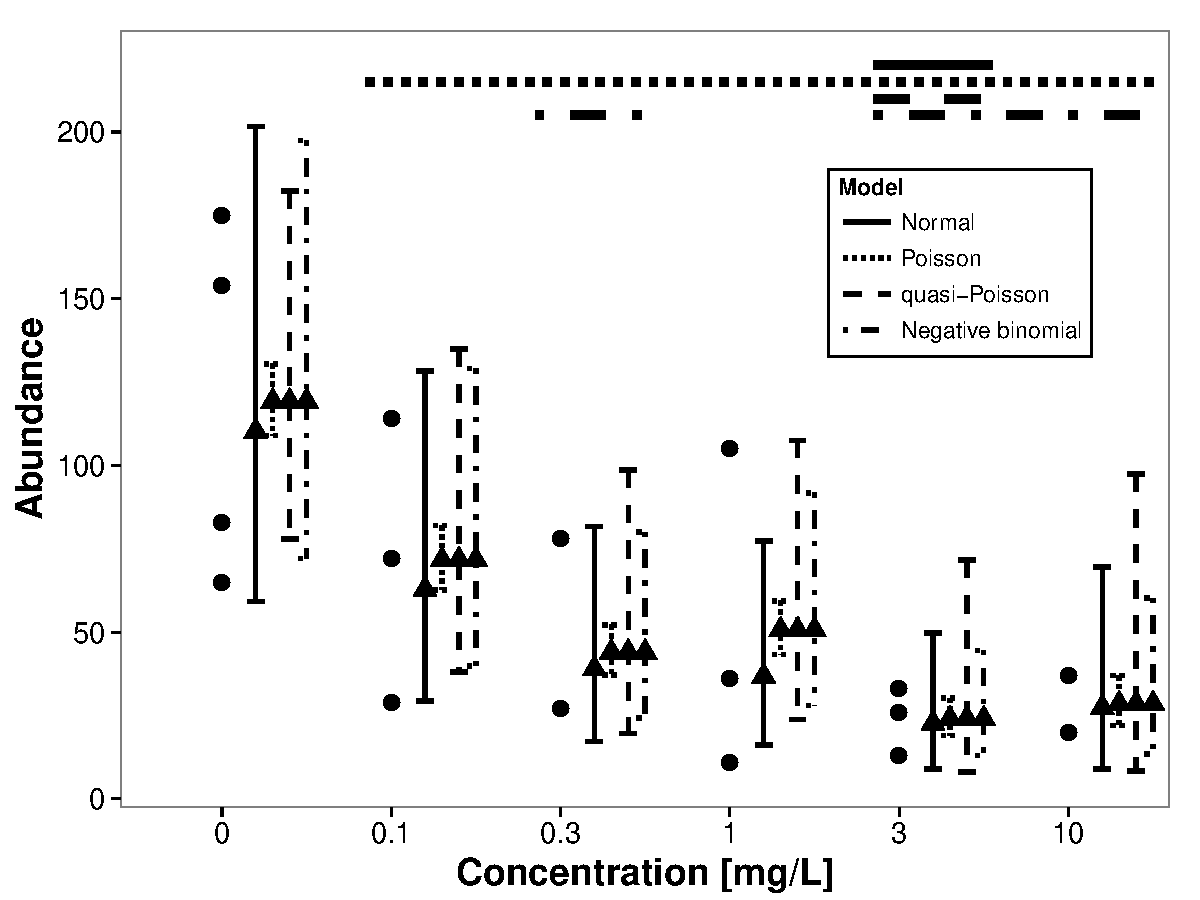
\includegraphics[width = 84mm]{example.pdf}
  \caption{Data from \citet{brock_minimum_2015} (dots). 
  Predicted values (triangles) and 95\% Wald Z or t confidence intervals from the fitted models (vertical lines) are given beside.
  Horizontal bars above indicate treatments statistically significant different from the control group (Dunnett contrasts).
  The data showed \DIFdelbeginFL \DIFdelFL{considerable }\DIFdelendFL overdispersion (\DIFdelbeginFL \DIFdelFL{$\Theta = 22.41$}\DIFdelendFL \DIFaddbeginFL \DIFaddFL{$\kappa = 4$}\DIFaddendFL ) and therefore, the Poisson model underestimates the \DIFaddbeginFL \DIFaddFL{width of }\DIFaddendFL confidence intervals.
  }
  \label{fig:example}
\end{figure}


%% --------------------------------
\subsection{Simulations}
\subsubsection{Count data}
To further scrutinise the differences between methods we simulated data sets with known properties.
We simulated count data that mimics the data of the case study with five treatments (T1 - T5) and one control group (C).
Counts were drawn from a negative binomial distribution with \DIFdelbegin \DIFdel{slight over dispersion }\DIFdelend \DIFaddbegin \DIFadd{overdispersion }\DIFaddend at all treatments (\DIFdelbegin \DIFdel{$\kappa = 0.25$}\DIFdelend \DIFaddbegin \DIFadd{$\kappa = 4$}\DIFaddend , eqn. \ref{eqn:negbin}).
We simulated data sets with different number of replicates (N = \{3, 6, 9\}) and different abundances in control treatments ($\mu_\text{\tiny C}$ = \{2, 4, 8, 16, 32, 64, 128\}). 
For power estimation, mean abundance in treatments T2 - T5 was reduced to half of control and T1 ($\mu_\text{\tiny T2}~=~...~=~\mu_\text{\tiny T5}~=~0.5~\mu_\text{\tiny C} = 0.5~\mu_\text{\tiny T1}$), resulting in a theoretical LOEC at T2.
Mean abundance was kept equal between all groups in Type 1 error simulations.
\DIFdelbegin %DIFDELCMD < 

%DIFDELCMD < %%%
\DIFdel{We generated 100 }\DIFdelend \DIFaddbegin \DIFadd{We generated 1000 }\DIFaddend data sets for each combination of N and $\mu_\text{\tiny C}$ and analysed these using the models outlined \DIFdelbegin \DIFdel{previously.
We did not fit Poisson models because we simulated data with overdispersion.
}\DIFdelend \DIFaddbegin \DIFadd{in section \ref{ssec:counts}.
}\DIFaddend 


\subsubsection{Binomial data}
We simulated data from a commonly used design as \DIFdelbegin \DIFdel{in }%DIFDELCMD < \citep{weber_short-term_1989}%%%
\DIFdelend \DIFaddbegin \DIFadd{described in }\citet{weber_short-term_1989}\DIFaddend , with 5 treated (T1 - T5) and a control group (C). 
Proportions were drawn from a Bin(10, $\pi$) distribution, with varying probability of survival (\DIFdelbegin \DIFdel{$\pi$ }\DIFdelend \DIFaddbegin \DIFadd{$\pi_C$ }\DIFaddend = \{0.60, 0.65, 0.70, 0.75, 0.80, 0.85, 0.90, 0.95\}) and varying number of replicates (N = \{3, 6, 9\}).
For Type 1 error estimation, \DIFdelbegin \DIFdel{$\pi$ }\DIFdelend \DIFaddbegin \DIFadd{$\pi_C$ }\DIFaddend was held constant between groups.
For power estimation \DIFdelbegin \DIFdel{$\pi$ }\DIFdelend \DIFaddbegin \DIFadd{$\pi_C$ }\DIFaddend in C and T1 was fixed at 0.95 and was set to values between 0.6 and 0.95 for the treatments T2 - T5. 
For each combination we simulated \DIFdelbegin \DIFdel{250 data sets }\DIFdelend \DIFaddbegin \DIFadd{1000 data sets and analysed these using the models outlined in section \ref{ssec:bin}}\DIFaddend .

\subsection{Data Analysis}
We analysed the case study and the simulated data using the outlined methods.
We compared the methods and models in terms of Type 1 error (\DIFdelbegin \DIFdel{maintain a significance level of 0.05 }\DIFdelend \DIFaddbegin \DIFadd{detection of an effect }\DIFaddend when there is \DIFdelbegin \DIFdel{no effect}\DIFdelend \DIFaddbegin \DIFadd{none}\DIFaddend ) and power (\DIFaddbegin \DIFadd{ability to }\DIFaddend detect an effect when it is present).
\DIFdelbegin \DIFdel{All computations }\DIFdelend \DIFaddbegin 

\DIFadd{All simulations }\DIFaddend were done in R (Version 3.1.2) \citep{r_core_team_r:_2014} on \DIFdelbegin \DIFdel{a Linux machine}\DIFdelend \DIFaddbegin \DIFadd{an Amazon EC2 virtual Linux server (64bit, 15GB RAM, 8 cores, 2.8 GHz)}\DIFaddend .
Source code \DIFdelbegin \DIFdel{for }\DIFdelend \DIFaddbegin \DIFadd{to reproduce }\DIFaddend the simulations and \DIFdelbegin \DIFdel{analysis of the case study }\DIFdelend \DIFaddbegin \DIFadd{paper }\DIFaddend is available online at \url{https://github.com/EDiLD/usetheglm}.
\DIFaddbegin \DIFadd{Moreover, Supplement 2 provides worked examples of the data of }\citet{brock_minimum_2015} \DIFadd{and }\citet{weber_short-term_1989}\DIFadd{.
}\DIFaddend 



%% ----------------------------------------------------------------------------
\section{Results}
\label{sec:results}
%% --------------------------------
\subsection{Case study}
The data set showed considerable \DIFdelbegin \DIFdel{overdispersion }\DIFdelend \DIFaddbegin \DIFadd{higher variance then expected by the Poisson model }\DIFaddend ($\Theta = 22.41$, eqn. \ref{eqn:quasi}). 
Therefore, the Poisson model did not fit to this data and lead to underestimated standard errors and confidence intervals, as well as overestimated statistical significance (Figure \ref{fig:example}).
In this case, inferences on the Poisson model are not valid and we do not further discuss its results.
The normal (F = 2.57, p = 0.084) and quasi-Poisson model (F = 2.90, p = 0.061), as well as the Kruskal test (p =  0.145) did not show a statistically significant treatment effects.
By contrast, the LR test and parametric bootstrap of the negative binomial model indicated a treatment-related effect (LR = 13.99, p = 0.016, bootstrap: p = 0.042).

All methods predicted similar values, except the normal model predicting always lower abundances (Figure \ref{fig:example}). 
95\% confidence intervals (CI) where most narrow for the negative binomial model and widest for the quasi-Poisson model - especially at lower estimated abundances.
Consequently, the LOECs differed (Normal and quasi-Poisson: 3 mg/L, negative binomial: 0.3 mg/L).
The pairwise Wilcoxon test did not detect any treatment different from control.


%% --------------------------------
\subsection{Simulations}
\subsubsection{Count data}
For \DIFaddbegin \DIFadd{detecting a general treatment effect $GLM_{nb}$ and $GLM_{p}$ showed inflated type 1 error rates, whereas $KW$ was conservative at low sample sizes.
However, using parametric bootstrap for the negative binomial model ($GLM_{npb}$) resulted in an appropriate type 1 error rates.
For detecting a treatment effect $GLM_{npb}$ and $GLM_{qp}$ exhibited higher power than $LM$ and $KW$, the latter having least power (Figure \ref{fig:p_glob_c}).
For }\DIFaddend our simulation design (reduction in abundance by 50\%) a sample size per treatment of n = 9 was needed to achieve a power greater than 80\%.
\DIFdelbegin \DIFdel{For detecting a treatment effect $GLM_{nb}$, $GLM_{npb}$ and $GLM_{qp}$ exhibited higher power than $LM$ and $KW$, the latter having least power.
Type 1 error rate was inflated for $GLM_{nb}$, but this could be fixed by using parametric bootstrap.
KW was conservative at low sample sizes (Figure \ref{fig:p_glob_c}).
}\DIFdelend At small sample sizes (n = {3, 6}) and low abundances ($\mu_C$ = {2, 4}) many of the negative binomial models ($GLM_{nb}$ and $GLM_{npb}$) did not converge to a solution (convergence rate \textless \DIFdelbegin \DIFdel{80}\DIFdelend \DIFaddbegin \DIFadd{85}\DIFaddend \% of the simulations, Supplement 1). 

\begin{figure*}
  \centering
  \DIFdelbeginFL %DIFDELCMD < 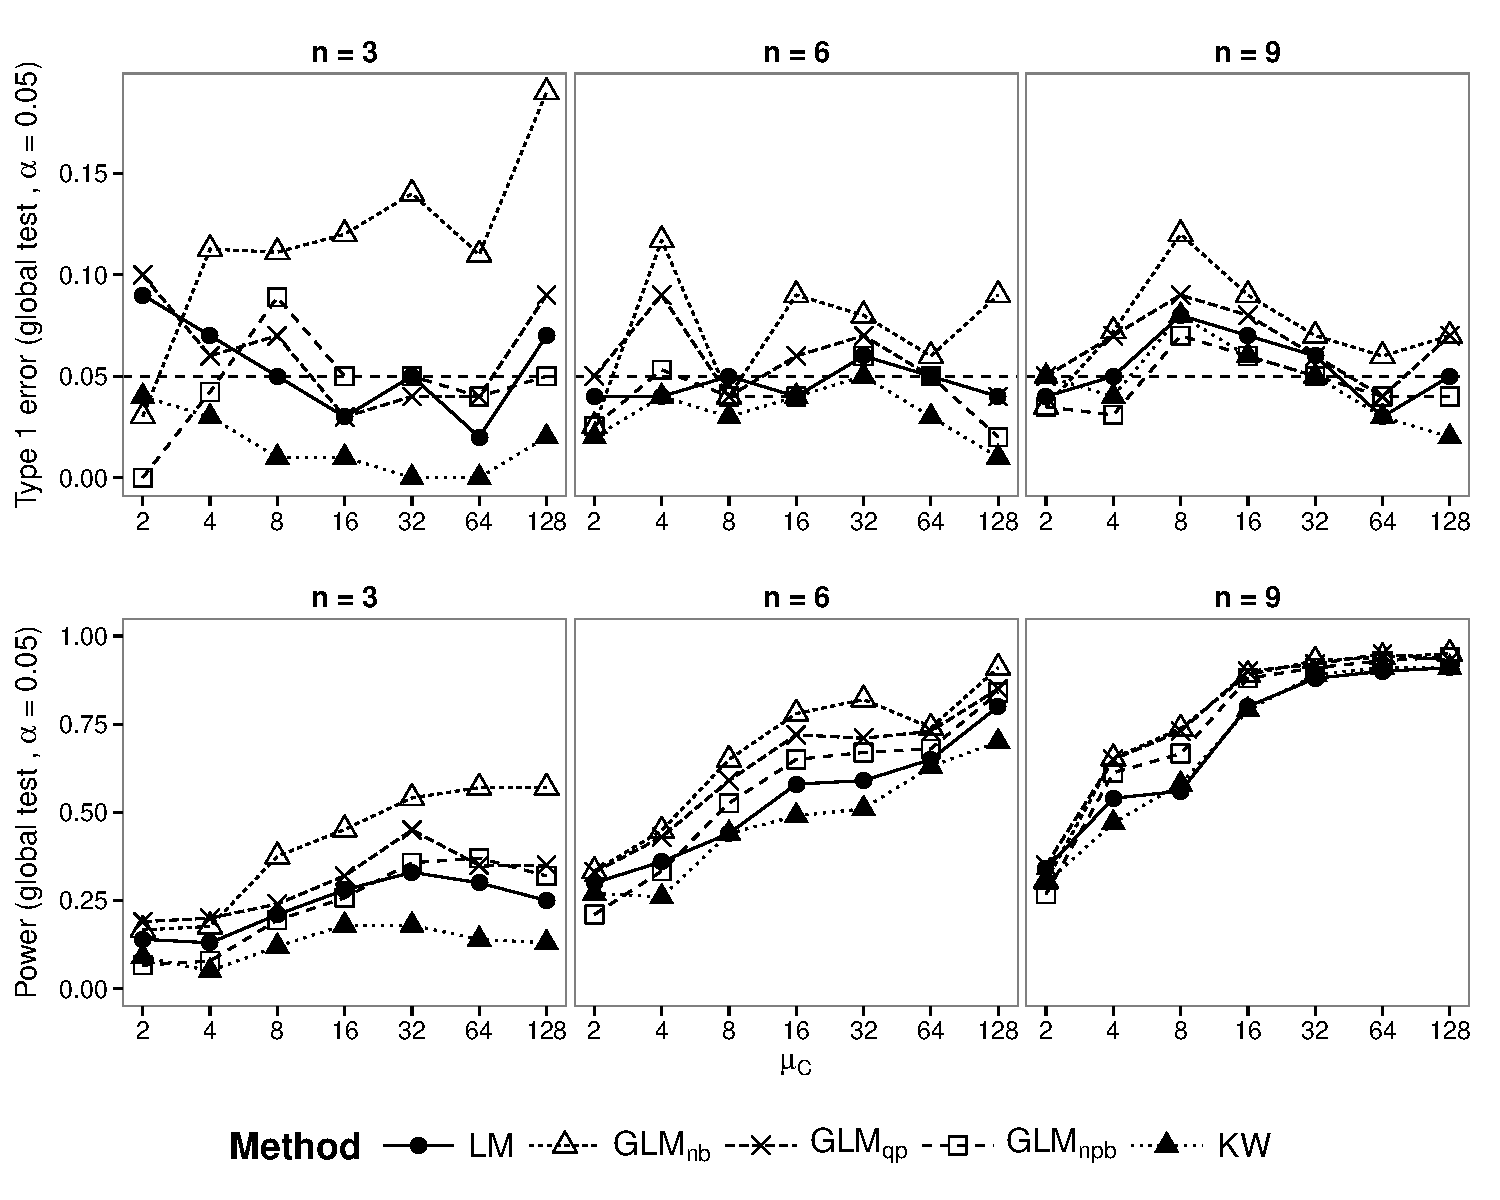
\includegraphics[width = 129mm]{p_glob_c.pdf}
%DIFDELCMD <   %%%
\DIFdelendFL \DIFaddbeginFL 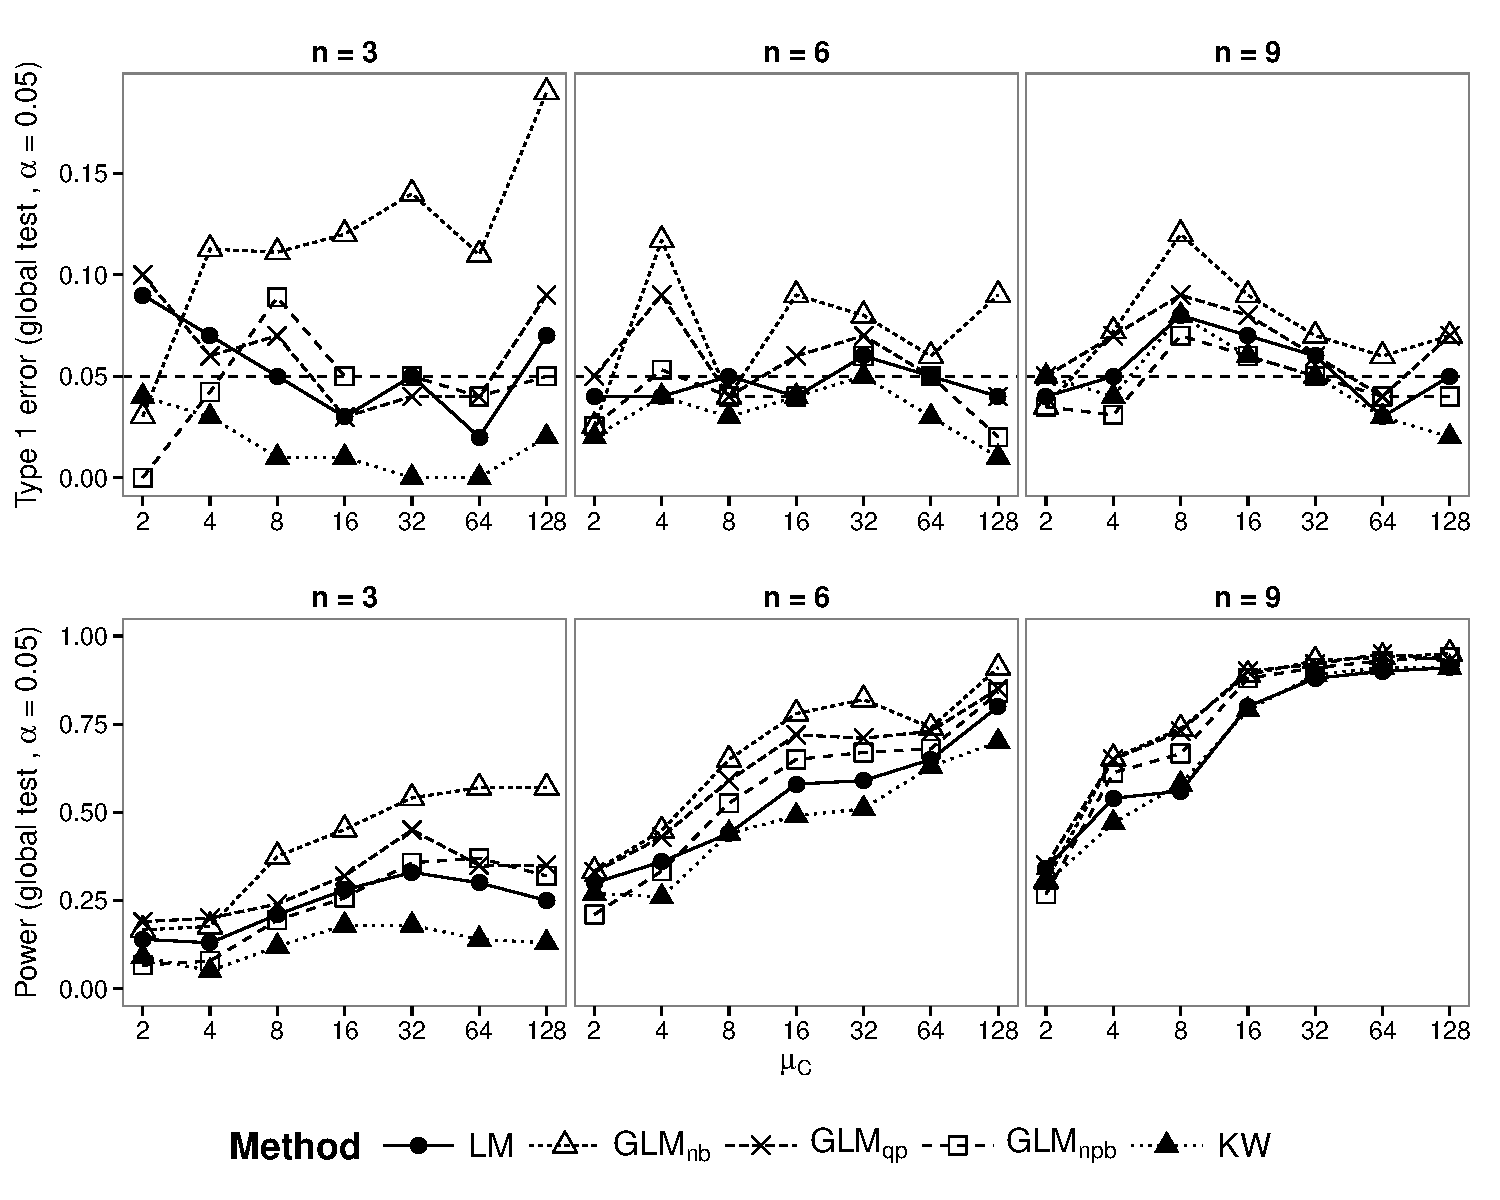
\includegraphics[width = 126mm]{p_glob_c.pdf}
  \DIFaddendFL \caption{Count data simulations: \DIFdelbeginFL \DIFdelFL{Power }\DIFdelendFL \DIFaddbeginFL \DIFaddFL{Type 1 error }\DIFaddendFL (top) and \DIFdelbeginFL \DIFdelFL{Type 1 error }\DIFdelendFL \DIFaddbeginFL \DIFaddFL{Power }\DIFaddendFL (bottom) for the test of a treatment effect.
  \DIFaddbeginFL \DIFaddFL{Only type 1 errors \textless 25\% are displayed. 
  $GLM_p$ showed type 1 errors \textgreater 20\% in all simulation scenarios.
  Power levels for models with inflated type I error are shown for completeness.
  }\DIFaddendFL For n = \DIFaddbeginFL \DIFaddFL{\{}\DIFaddendFL 3\DIFaddbeginFL \DIFaddFL{, 6\} }\DIFaddendFL and $\mu_C$ = \{2, 4\} less than \DIFdelbeginFL \DIFdelFL{80}\DIFdelendFL \DIFaddbeginFL \DIFaddFL{85}\DIFaddendFL \% of $GLM_{nb}$ and $GLM_{npb}$ models did converge.
  Dashed horizontal line denotes the nominal Type 1 error rate at $\alpha = 0.05$.
  }
  \label{fig:p_glob_c}
\end{figure*}

\DIFaddbegin \DIFadd{For LOEC determination $GLM_{nb}$ and $GLM_{p}$ showed an increased Type 1 error and all other methods being slightly conservative.
}\DIFaddend The inferences on LOEC generally showed less power.
\DIFdelbegin \DIFdel{For }\DIFdelend $LM$ \DIFdelbegin \DIFdel{this reduction was up to 35\% compared to the overall treatment effect (n = 9, $\mu_C$ = 64, Figures \ref{fig:p_glob_c} and \ref{fig:p_loec_c}).
The power }\DIFdelend \DIFaddbegin \DIFadd{showed a mean reduction of 20.7\% and $GLM_{qp}$ of 24.3 \%.
Power }\DIFaddend to detect the LOEC was highest for \DIFdelbegin \DIFdel{$GLM_{nb}$ and $GLM_{npb}$}\DIFdelend \DIFaddbegin \DIFadd{$GLM_{qp}$}\DIFaddend . 
$LM$ and \DIFdelbegin \DIFdel{WT }\DIFdelend \DIFaddbegin \DIFadd{$WT$ }\DIFaddend showed less power, with \DIFdelbegin \DIFdel{WT }\DIFdelend \DIFaddbegin \DIFadd{$WT$ }\DIFaddend having no power to detect the LOEC at low sample sizes \DIFdelbegin \DIFdel{.
At low sample sizes $GLM_{nb}$ showed an increased Type 1 error and WT was slightly conservative }\DIFdelend (Figure \ref{fig:p_loec_c}).

\begin{figure*}
  \centering
  \DIFdelbeginFL %DIFDELCMD < 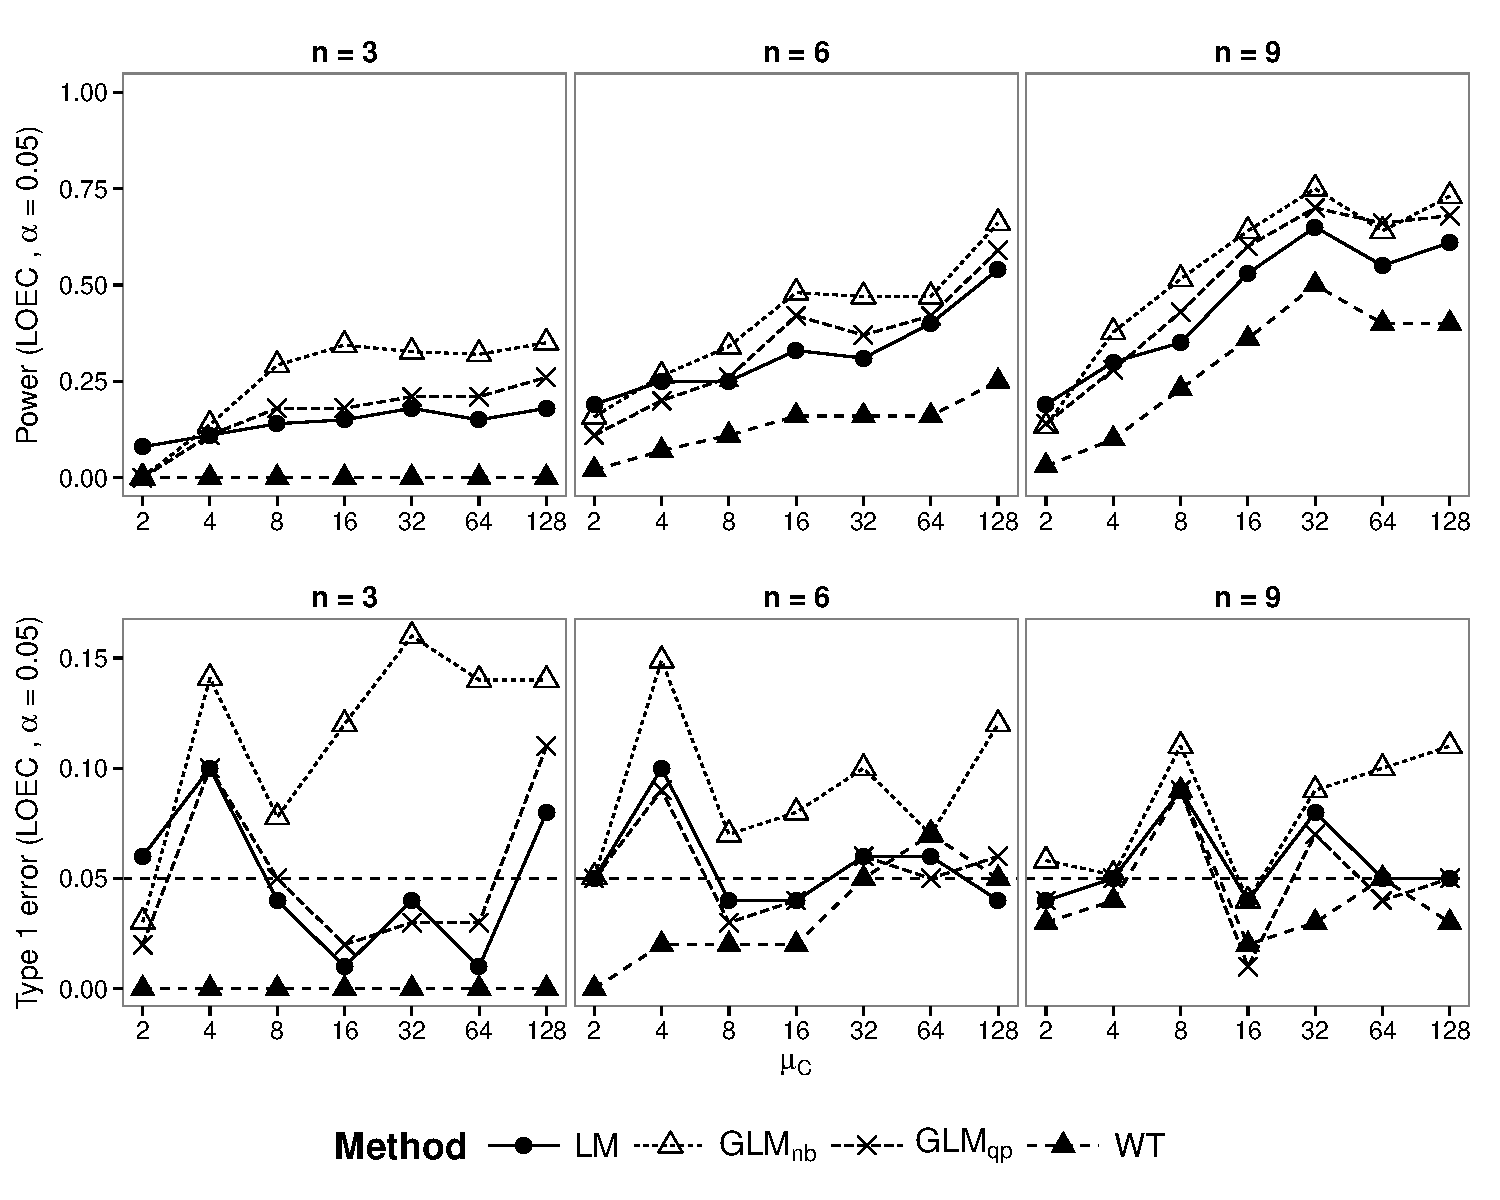
\includegraphics[width = 129mm]{p_loec_c.pdf}
%DIFDELCMD <   %%%
\DIFdelendFL \DIFaddbeginFL 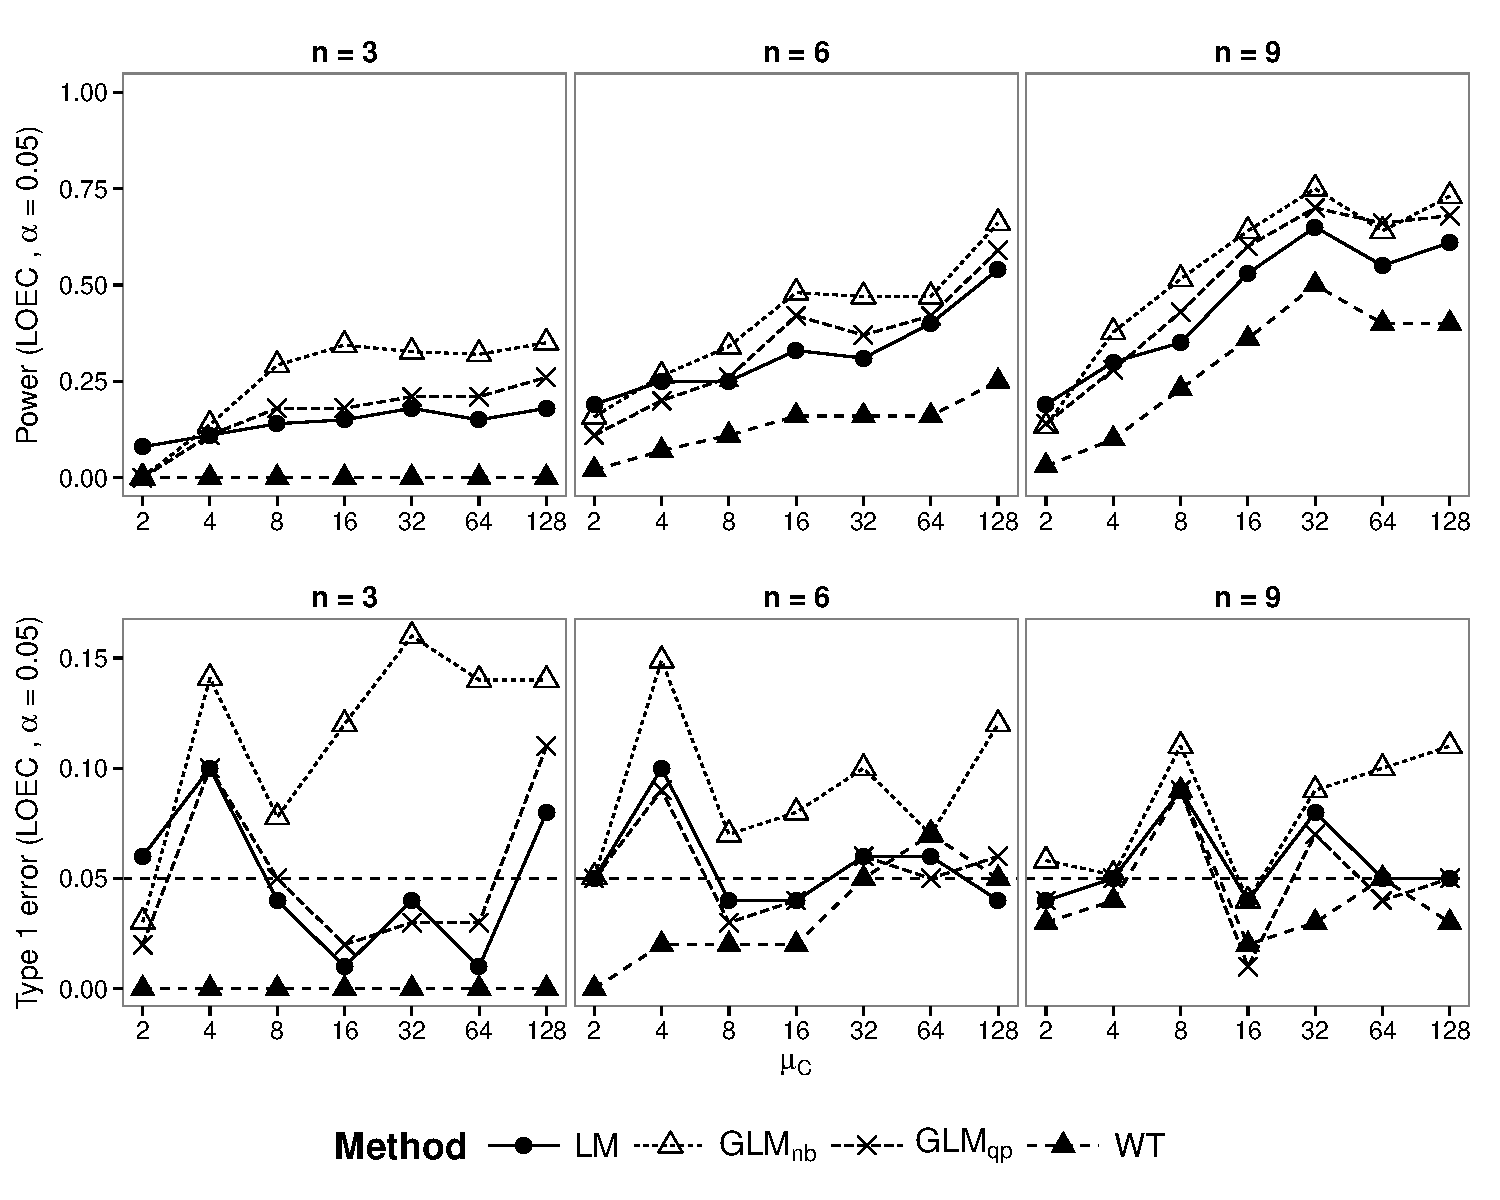
\includegraphics[width = 126mm]{p_loec_c.pdf}
  \DIFaddendFL \caption{Count data simulations: \DIFdelbeginFL \DIFdelFL{Power }\DIFdelendFL \DIFaddbeginFL \DIFaddFL{Type 1 error }\DIFaddendFL (top) and \DIFdelbeginFL \DIFdelFL{Type 1 error }\DIFdelendFL \DIFaddbeginFL \DIFaddFL{Power }\DIFaddendFL (bottom) for determination of LOEC.
  For \DIFaddbeginFL \DIFaddFL{clarity only type 1 errors \textless 25\% are displayed.
  Power levels for models with inflated type I error are shown for completeness.
  For }\DIFaddendFL n = \DIFaddbeginFL \DIFaddFL{\{}\DIFaddendFL 3\DIFaddbeginFL \DIFaddFL{, 6\} }\DIFaddendFL and $\mu_C$ = \{2, 4\} less than \DIFdelbeginFL \DIFdelFL{80}\DIFdelendFL \DIFaddbeginFL \DIFaddFL{85}\DIFaddendFL \% of $GLM_{nb}$ \DIFdelbeginFL \DIFdelFL{and $GLM_{npb}$ }\DIFdelendFL models did converge.
  Dashed horizontal line denotes the nominal Type 1 error rate at $\alpha = 0.05$.
  }
  \label{fig:p_loec_c}
\end{figure*}


\subsubsection{Binomial data}
\DIFaddbegin 

\DIFaddend $GLM_{bin}$ showed \DIFaddbegin \DIFadd{slightly increased type 1 error rates at low sample sizes and small effect sizes.
$KW$ was more conservative than $LM$ and $GLM_{bin}$.
$GLM_{bin}$ showed }\DIFaddend the greatest power for testing the treatment effect. 
This was especially apparent at low sample sizes (n = 3), with up to \DIFdelbegin \DIFdel{24}\DIFdelend \DIFaddbegin \DIFadd{27}\DIFaddend \% higher power compared to LM.
\DIFdelbegin \DIFdel{KW had the lowest power and was slightly conservative.
}\DIFdelend However, the differences between methods quickly vanished with increasing samples sizes \DIFdelbegin \DIFdel{. 
KW was more conservative than LM and $GLM_{bin}$ }\DIFdelend (Figure \ref{fig:p_glob_p}).

\begin{figure*}
  \centering
  \DIFdelbeginFL %DIFDELCMD < 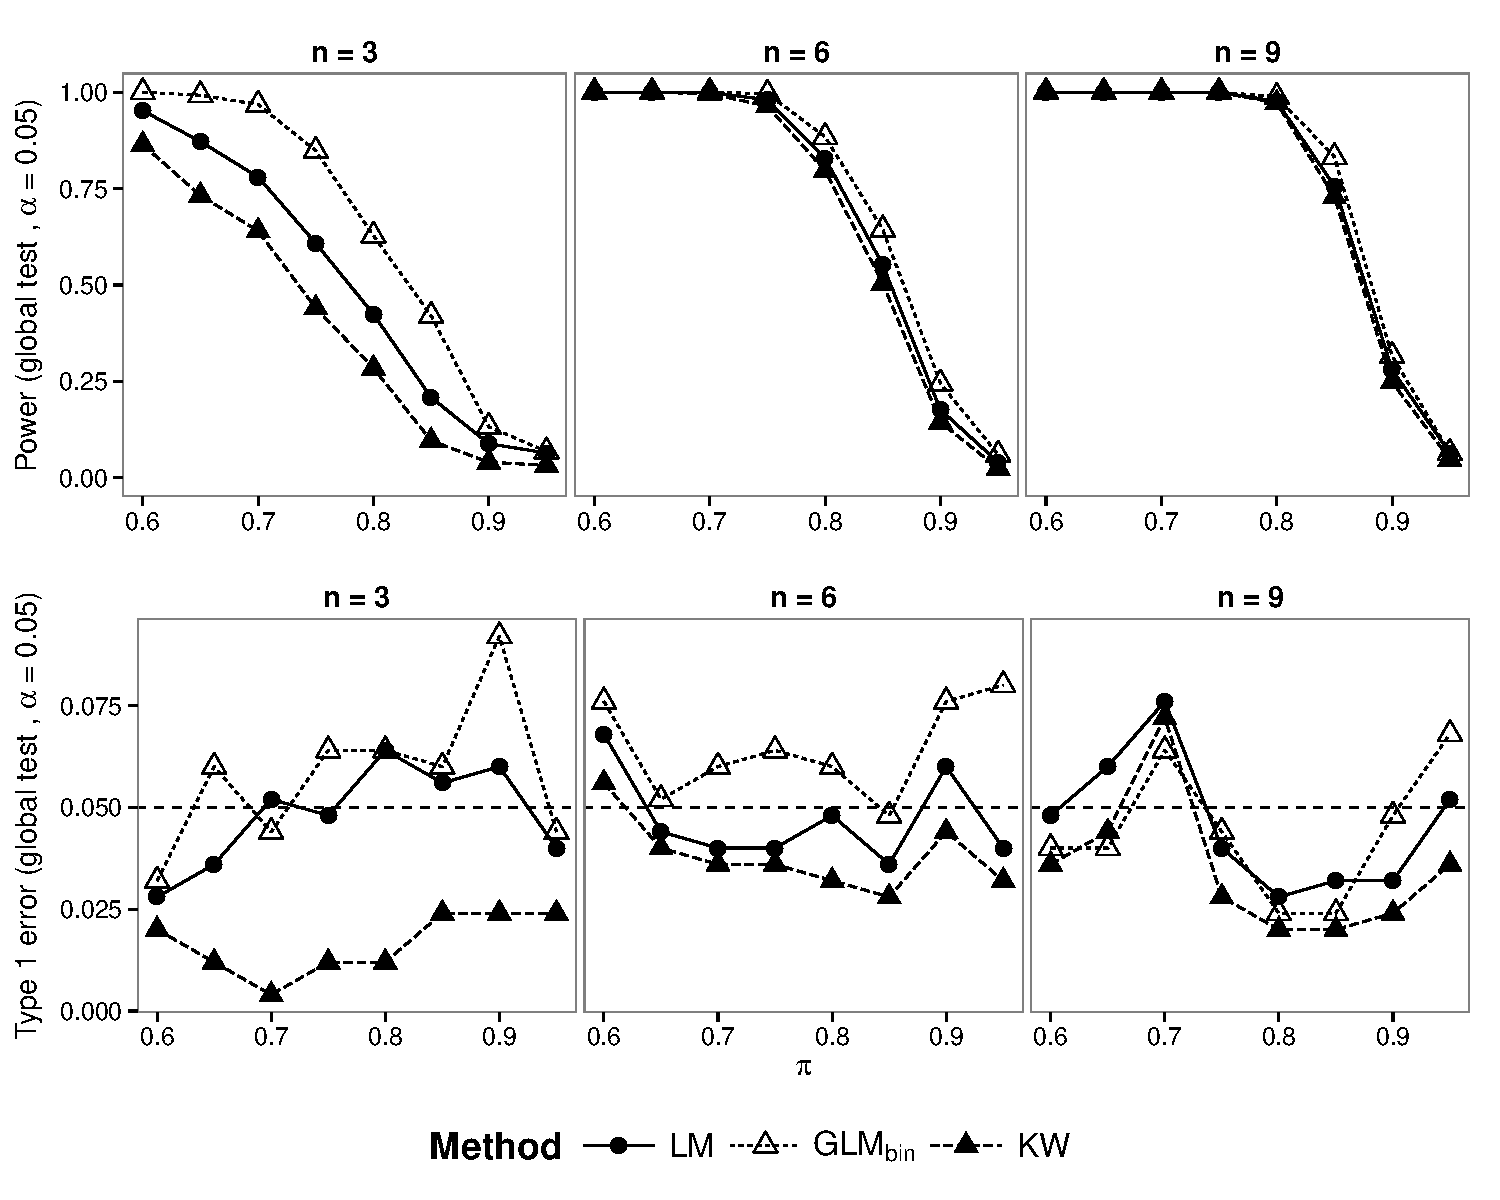
\includegraphics[width = 129mm]{p_glob_p.pdf}
%DIFDELCMD <   %%%
\DIFdelendFL \DIFaddbeginFL 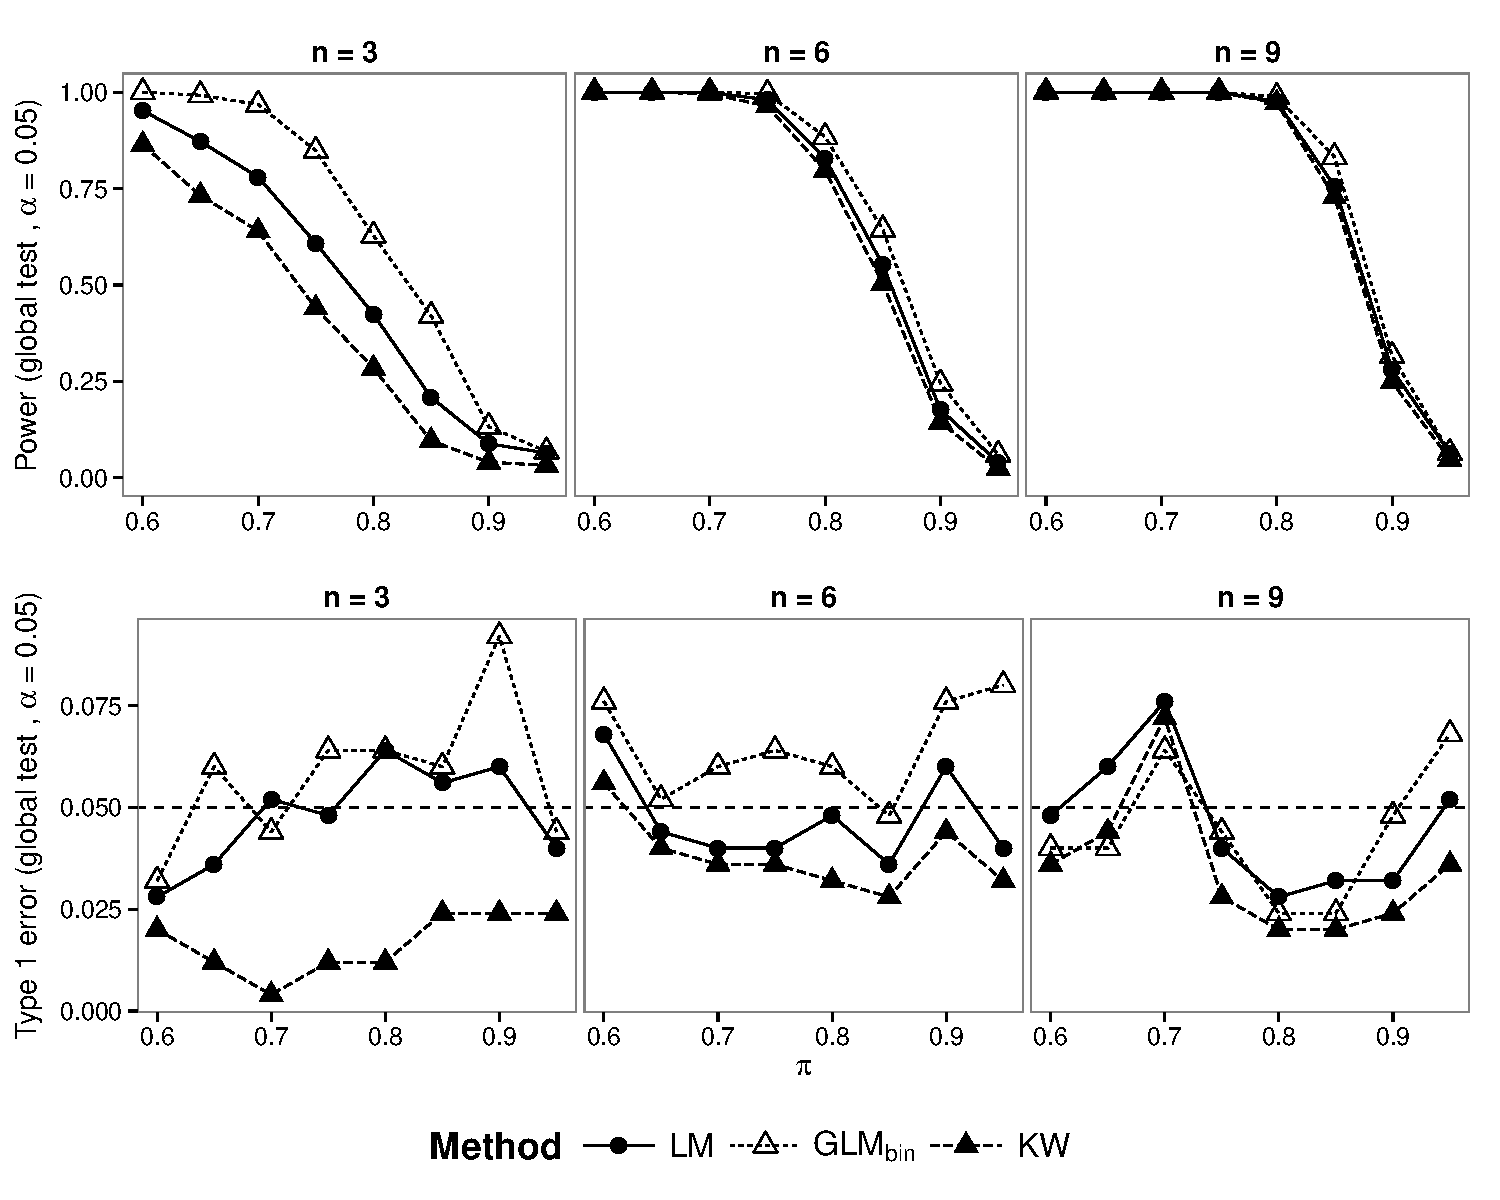
\includegraphics[width = 126mm]{p_glob_p.pdf}
  \DIFaddendFL \caption{
  Binomial data simulations: 
  \DIFdelbeginFL \DIFdelFL{Power }\DIFdelendFL \DIFaddbeginFL \DIFaddFL{Type 1 error }\DIFaddendFL (top) and  \DIFdelbeginFL \DIFdelFL{Type 1 error }\DIFdelendFL \DIFaddbeginFL \DIFaddFL{power }\DIFaddendFL (bottom) for the test of a treatment effect. 
  Dashed horizontal line denotes the nominal Type 1 error rate at $\alpha = 0.05$.
  }
  \label{fig:p_glob_p}
\end{figure*}

\DIFaddbegin \DIFadd{For inference on LOEC we found that all methods were slightly conservative.
$WT$ was generally more conservative and $GLM_{bin}$ especially at low effect sizes ($p_E > 0.7$).
}\DIFaddend Inference on LOEC was not as powerful as inference on the general treatment effect.
Contrary to the general treatment effect, $LM$ showed the higher power than $GLM_{bin}$ at small sample sizes \DIFdelbegin \DIFdel{.
However, these differences in power were only apparent at }\DIFdelend \DIFaddbegin \DIFadd{(}\DIFaddend n = \DIFaddbegin {\DIFaddend 3\DIFdelbegin \DIFdel{and vanished quickly with increasing sample sizes (Figure \ref{fig:p_loec_p}).
WT }\DIFdelend \DIFaddbegin \DIFadd{, 6}}\DIFadd{).
$WT$ }\DIFaddend had no power for n = 3 and showed less power in the other simulation runs \DIFdelbegin \DIFdel{.
$LM$ maintained a Type 1 error level of 0.05 in all simulations. 
$GLM_{bin}$ was conservative at small effect sizes ($p_E > 0.8$) and WT was generally conservative showing lowered Type 1 error rates (}\DIFdelend \DIFaddbegin \DIFadd{(}\DIFaddend Figure \ref{fig:p_loec_p}).

\DIFdelbegin %DIFDELCMD < \begin{figure}
%DIFDELCMD <   %%%
\DIFdelendFL \DIFaddbeginFL \begin{figure*}
  \DIFaddendFL \centering
  \DIFdelbeginFL %DIFDELCMD < 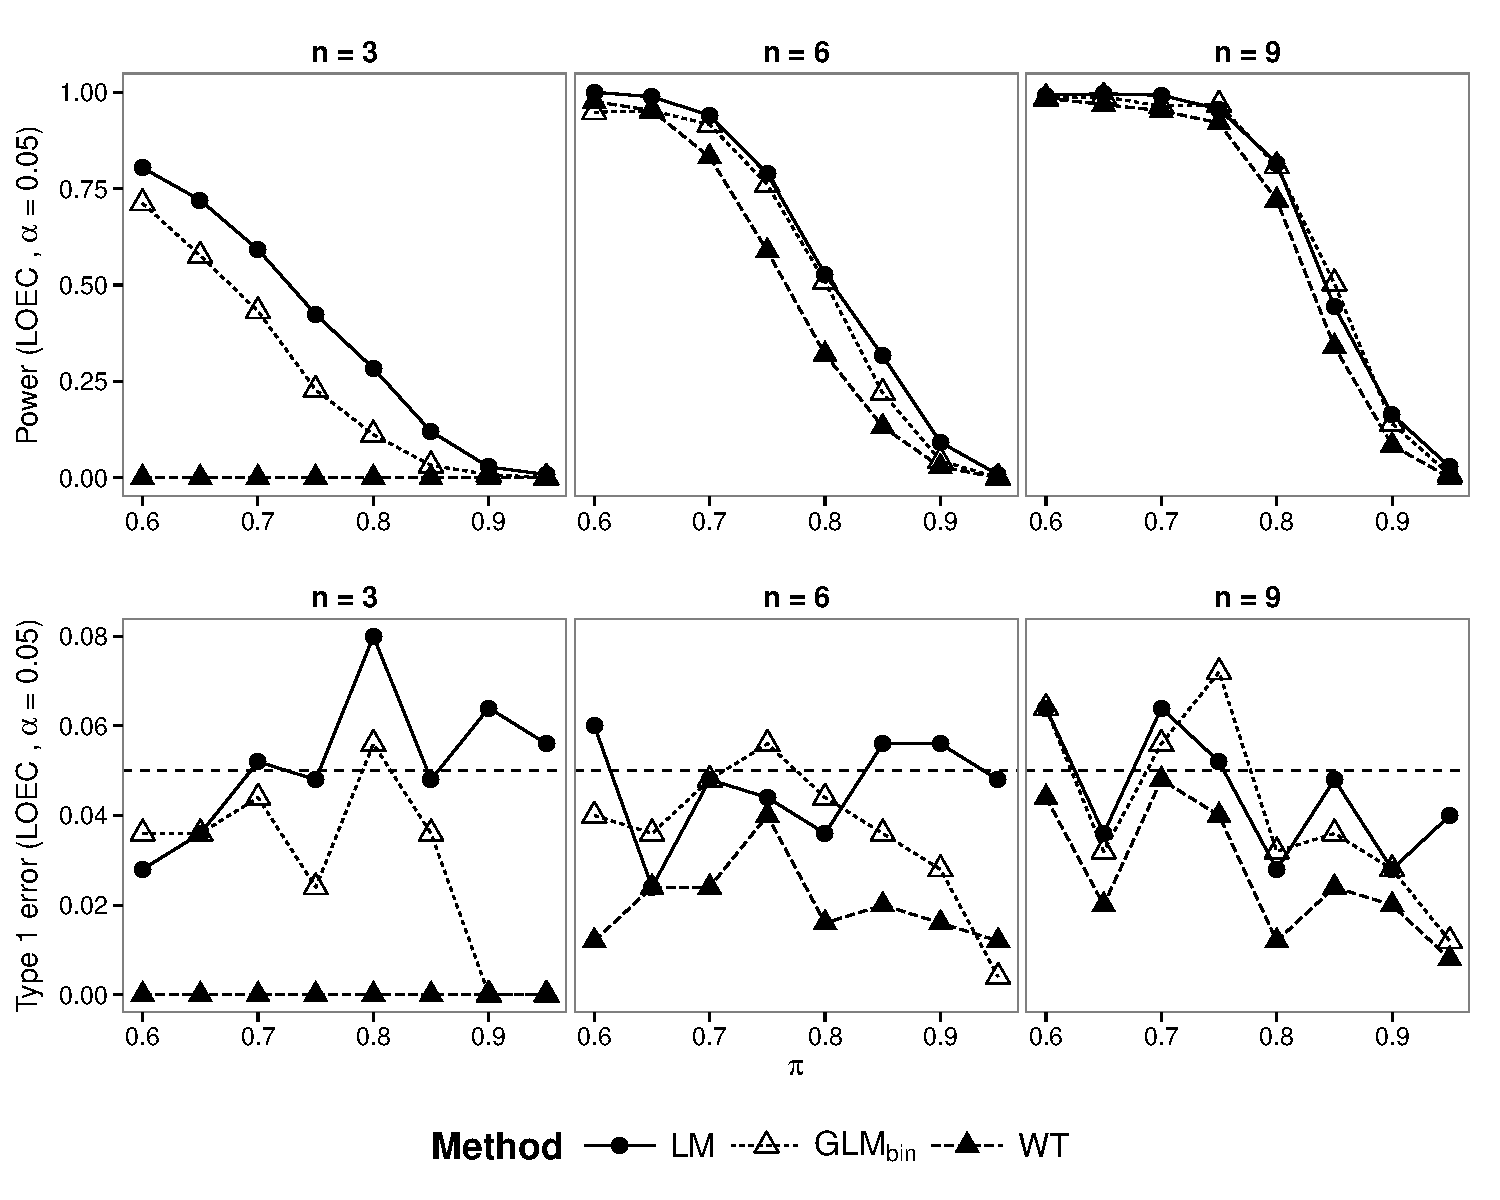
\includegraphics[width = 84mm]{p_loec_p.pdf}
%DIFDELCMD <   %%%
\DIFdelendFL \DIFaddbeginFL 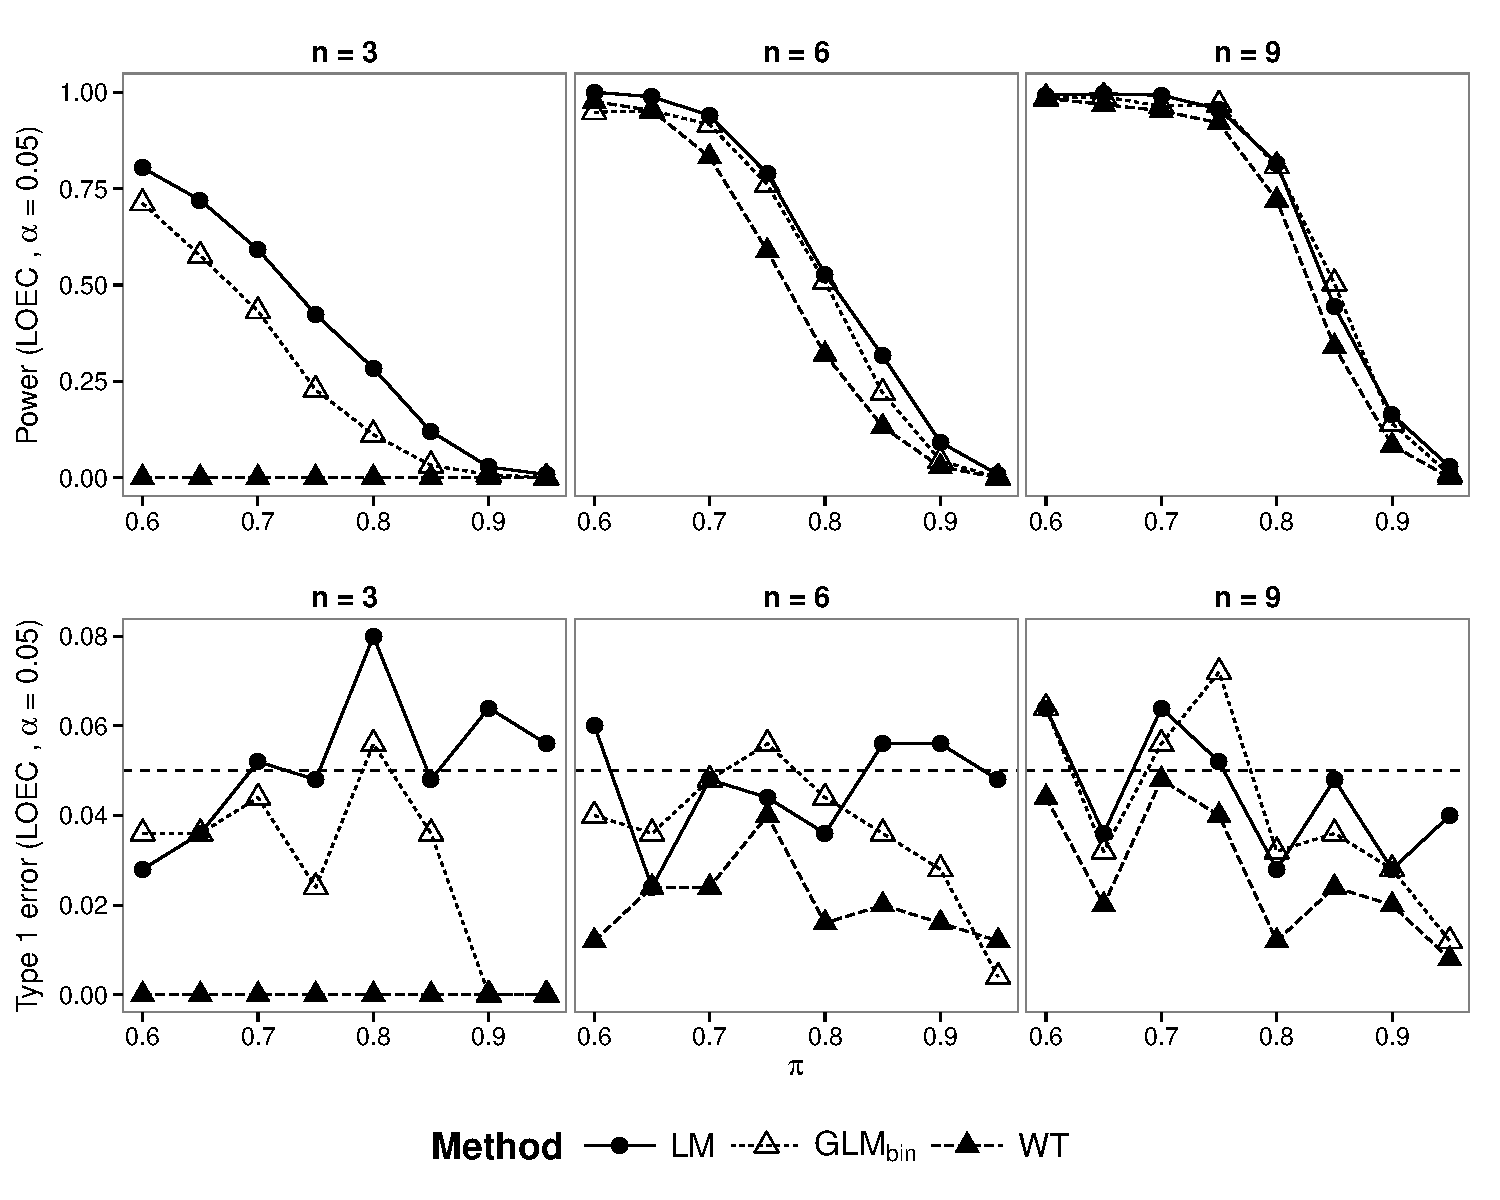
\includegraphics[width = 126mm]{p_loec_p.pdf}
  \DIFaddendFL \caption{
  Binomial data simulations: 
  \DIFdelbeginFL \DIFdelFL{Power }\DIFdelendFL \DIFaddbeginFL \DIFaddFL{Type 1 error }\DIFaddendFL (top) and \DIFdelbeginFL \DIFdelFL{Type 1 error }\DIFdelendFL \DIFaddbeginFL \DIFaddFL{power }\DIFaddendFL (bottom) for the test for determination of LOEC. 
  Dashed horizontal line denotes the nominal Type 1 error rate at $\alpha = 0.05$.
  }
  \label{fig:p_loec_p}
\DIFdelbeginFL %DIFDELCMD < \end{figure}
%DIFDELCMD < %%%
\DIFdelend \DIFaddbegin \end{figure*}
\DIFaddend 


%% ----------------------------------------------------------------------------
\section{Discussion}
\label{sec:disc}
\subsection{Case study}
%% ---- Case study
The outlined case study demonstrates that the choice of the statistical model and procedure can have substantial impact on ecotoxicological inferences and endpoints like the LOEC.
\DIFaddbegin \DIFadd{Therefore, ecotoxicologists should not base their inferences solely on statistical significance tests, but also on parameter estimates, their uncertainty and importance }\citep{gelman_difference_2006}\DIFadd{.
Nevertheless, }\citet{ohara_not_2010} \DIFadd{showed that $LM$ using a log transformation gave unreliable and biased parameter estimates, whereas GLMs performed well with little bias.
Bias occurs also when back-transforming means to the original scale, which explains the lower predicted means by $LM$ in Figure \ref{fig:example} }\citep{rothery_cautionary_1988} \DIFadd{and should be corrected for }\citep{newman_regression_1993}\DIFadd{.
}

\DIFaddend This is further highlighted by the fact that for the same model (linear model of transformed data), \citet{brock_minimum_2015} reported a 10-fold lower LOEC (\mbox{0.3 mg/L}) then found in our study (3 mg/L, Figure \ref{fig:example}).
The reasons are be manifold: \citep{brock_minimum_2015} used a $log(2~y + 1)$ transformation, whereas we used a $log(A~y + 1)$ transformation, where A = 2 / 11 = 0.182 \citep{van_den_brink_impact_2000}.
\DIFdelbegin \DIFdel{Furthermore, }\DIFdelend \DIFaddbegin \DIFadd{However, this contributed only little to the differences.
A much bigger impact had the type of multiple comparison: }\DIFaddend \citet{brock_minimum_2015} used a one-sided Williams test\DIFdelbegin \DIFdel{which assumes a monotonic dose-response relationship.
In contrast, we used a }\DIFdelend \DIFaddbegin \DIFadd{, whereas we used }\DIFaddend one-sided \DIFdelbegin \DIFdel{Dunnett test, which does not assume monotonicity }\DIFdelend \DIFaddbegin \DIFadd{comparisons to the control (Dunnett contrasts).
In contrast to the Williams type contrasts, Dunnett contrasts do not assume a monotonic dose-response relationship }\DIFaddend and allows individual comparisons between treatment groups and the control\DIFaddbegin \DIFadd{.
However}\DIFaddend , but has under monotonicity \DIFdelbegin \DIFdel{less power }\DIFdelend \DIFaddbegin \DIFadd{they have less power which explain the differences }\DIFaddend \citep{jaki_statistical_2013}.
\DIFaddbegin \DIFadd{Both contrasts are available in a GLM framework.
Therefore, the choice of contrast depends on the assumptions one to make and which questions to answer. 
However, it this should affect our comparisons between methods.
}\DIFaddend 

%% ---- Guide GLMs
\DIFdelbegin \DIFdel{Moreover, }\DIFdelend \DIFaddbegin \DIFadd{Overdispersion is common with ecological datasets }\citep{warton_many_2005} \DIFadd{and }\DIFaddend the case study illustrates the potential effects of overdispersion that is not accounted for: standard \DIFdelbegin \DIFdel{error }\DIFdelend \DIFaddbegin \DIFadd{errors }\DIFaddend will be underestimated and significance overestimated (\DIFdelbegin \DIFdel{Figure }\DIFdelend \DIFaddbegin \DIFadd{Figures }\DIFaddend \ref{fig:example}).
\DIFaddbegin \DIFadd{This is also shown by our simulations (Figures \ref{fig:p_glob_c}, \ref{fig:p_loec_c}) where $GLM_p$ showed increased type 1 error rates because of overdispersed simulated data. 
}\DIFaddend However, in factorial designs the mean-variance relationship can be easily checked by plotting mean versus variance of the treatment groups (see \DIFdelbegin \DIFdel{supplemental material}\DIFdelend \DIFaddbegin \DIFadd{Supplement 2}\DIFaddend ).
In the introduction we pointed out that there is little advice how to choose between the plenty of possible transformations - how do GLMs simplify this problem?
The distribution modelled can be chosen \DIFdelbegin \DIFdel{by the nature of the data giving a statistically sound model reflecting its properties }\DIFdelend \DIFaddbegin \DIFadd{using knowledge about the data }\DIFaddend (e.g. \DIFdelbegin \DIFdel{bonds}\DIFdelend \DIFaddbegin \DIFadd{bounds}\DIFaddend , integer or continuous data etc\DIFdelbegin \DIFdel{.}\DIFdelend ).
Knowing what type of data is modelled (see Methods section), the model selection process can be completely guided by the data and diagnostic \DIFdelbegin \DIFdel{plots}\DIFdelend \DIFaddbegin \DIFadd{tools}\DIFaddend . Therefore, choosing an appropriate model is \DIFdelbegin \DIFdel{more sound and straightforward }\DIFdelend \DIFaddbegin \DIFadd{easier }\DIFaddend than choosing between possible transformations.


\subsection{Simulations}
%% --- general low power
Our simulations showed that generally GLMs have greater power than data transformations.
However, the simulations also suggest that the power at the population level in common mesocosm experiments is low.
For common samples sizes and a reduction in abundance of 50\% we found a low power to detect any treatment-related effect (\textless 50\% for methods with appropriate Type 1 error, Figure \ref{fig:p_glob_c}).
\DIFdelbegin \DIFdel{Additionally, }%DIFDELCMD < \citet{ohara_not_2010} %%%
\DIFdel{showed that using a log transformation gave unreliable and biased parameter estimates.
}\DIFdelend Statistical power to detect the correct LOEC was even lower (less than 30\%)\DIFdelbegin \DIFdel{.
This }\DIFdelend \DIFaddbegin \DIFadd{, which can be attributed to multiple testing.
The low power of all methods for detecting the LOEC }\DIFaddend suggests that population level NOECs reported from mesocosm experiments should be interpreted with caution and underpins the criticism of NOEC \citep{laskowski_good_1995,landis_well_2011}.

%% --- Multivariate + GLMM -------
Mesocosm studies allow also inferences on community level. 
For community analyses \emph{GLM for multivariate data} \DIFaddbegin \citep{warton_distance-based_2012} \DIFaddend have been proposed as alternative to Principal Response Curves (PRC) and yielded to similar inferences, but better indication of responsive taxa \DIFdelbegin %DIFDELCMD < \citep{warton_distance-based_2012,szocs_analysing_2015}%%%
\DIFdel{. 
}\DIFdelend \DIFaddbegin \citep{szocs_analysing_2015}\DIFadd{. 
However, }\citet{ter_braak_topics_2014} \DIFadd{argue to use data transformations with community data because of their easy- and robustness.
}\DIFaddend Although our simulations covered only simple experimental designs at the population level, findings may also extend to more complex situations. 
Nested or repeated designs with non-normal data could be analysed using Generalised Linear Mixed Models (GLMM) and may have advantages with respect to power \citep{stroup_rethinking_2014}.

%% --- Alternatives -------
To counteract the problems with low power at the population level \citet{brock_minimum_2015} proposed to take the Minimum Detectable Difference (MDD), a method to assess statistical power \emph{a posteriori}, for inference into account.
However, \emph{a \DIFdelbegin \DIFdel{priory}\DIFdelend \DIFaddbegin \DIFadd{priori}\DIFaddend } power analyses can be performed easily using simulations, even for complex experimental designs \citep{johnson_power_2014}, and might help to design, interpret and evaluate ecotoxicological studies.
Moreover, \citet{brock_minimum_2015} proposed that statistical power of mesocosm experiments can be increased by reducing sampling variability through improved sampling techniques and quantification methods, though they also caution against depleting populations through more exhaustive sampling.
As we showed, using appropriate statistical methods (like GLMs) can enhance the power at no extra costs.

%% --- Non-parametric
\citet{wang_making_2011} advocated that in the typical case of small sample sizes (n \textless 20) and non-normal data, non-parametric tests perform better than parametric tests assuming normality.
In contrast, our results showed that the often applied \DIFdelbegin \DIFdel{Kruskal test and pairwise Wilcoxon test have equal or }\DIFdelend \DIFaddbegin \DIFadd{$KW$ and $WT$ have }\DIFaddend less power compared to \DIFdelbegin \DIFdel{tests assuming normality after data transformation}\DIFdelend \DIFaddbegin \DIFadd{$LM$}\DIFaddend .
Moreover, \DIFdelbegin \DIFdel{GLMs }\DIFdelend \DIFaddbegin \DIFadd{$GLMs$ }\DIFaddend always performed better than non-parametric tests. 
Though more powerful non-parametric tests may be available \citep{konietschke_rank-based_2012}, these are focused on hypothesis testing and do not provide estimation of effect sizes.
Additionally to testing, GLMs allow the estimation and interpretation of effects that might not be statistically significant, but ecologically relevant.
Therefore, we advise using GLMs instead of non-parametric tests for non-normal data.

%% ---- Problems GLM
\DIFdelbegin \DIFdel{At }\DIFdelend \DIFaddbegin \DIFadd{We found an increased Type-I error for $GLM_{nb}$ at low sample sizes.
However, it is well known that the LR statistic is not reliable at }\DIFaddend small sample sizes \DIFdelbegin \DIFdel{and }\DIFdelend \DIFaddbegin \citep{bolker_generalized_2009,wilks_large-sample_1938}\DIFadd{.
Parametric bootstrap ($GLM_{npb}$) is a valuable alternative in such situations and maintains appropriate levels (Figure \ref{fig:p_glob_c}).
Moreover, at small sample sizes and }\DIFaddend low abundances a significant amount of negative binomial models did not converge.
We used an iterative algorithm to fit these models \citep{venables_modern_2002}and other methods assessing the likelihood directly may perform better.
\DIFdelbegin \DIFdel{Moreover, the Likelihood-Ratio test gave an increased Type-I error for these models, where the non reliability of the LR statistic for small sample sizes has long been reported }%DIFDELCMD < \citep{bolker_generalized_2009,wilks_large-sample_1938}%%%
\DIFdel{. 
We found that parametric bootstrap (}\DIFdelend \DIFaddbegin 

\DIFadd{$GLM_{qp}$ showed higher statistical power than }\DIFaddend $GLM_{npb}$ \DIFdelbegin \DIFdel{) provides a valuable alternative in such situations }\DIFdelend (Figure \ref{fig:p_glob_c}\DIFdelbegin \DIFdel{).
At }\DIFdelend \DIFaddbegin \DIFadd{, bottom).
This could be explained by the simpler mean-variance relationship of $GLM_{qp}$ (eqn. \ref{eqn:quasi} and \ref{eqn:negbin}), because at }\DIFaddend small samples sizes, low abundances or few treatment groups it is difficult to determine the mean-variance relationship.
\DIFdelbegin \DIFdel{$GLM_{qp}$ assumes a simpler, linear mean-variance relationship, which might explain the higher power compared to $GLM_{npb}$ at small sample sizes (Figure \ref{fig:p_glob_c}, top).
}\DIFdelend 

%% --- binomial data
Binomial data \DIFdelbegin \DIFdel{is }\DIFdelend \DIFaddbegin \DIFadd{are }\DIFaddend often collected in lab trials, where increasing the sample size is easy to accomplish. 
We found notable differences in power to detect a treatment effect \DIFdelbegin \DIFdel{up to a sample size of 9.
}\DIFdelend \DIFaddbegin \DIFadd{for all simulated sample sizes.
}\DIFaddend Similarly, \citet{warton_arcsine_2011} also found that \DIFdelbegin \DIFdel{GLM }\DIFdelend \DIFaddbegin \DIFadd{GLMs }\DIFaddend have higher power than arcsine transformed linear models.
\DIFdelbegin \DIFdel{Nevertheless, for deriving LOECs the transformation performed better }\DIFdelend \DIFaddbegin \DIFadd{Though we did not simulated overdispersed binomial data, this should be checked and accounted for.
In such situations a GLMM may offer an appealing alternative }\citep{warton_arcsine_2011}\DIFadd{.
At low effect sizes $GLM_{bin}$ became conservative with increasing $\pi_C$, although this effect lessened as sample size increased (Figure \ref{fig:p_loec_p}). 
This is because $\pi$ approaches its boundary and is also known as the }\emph{\DIFadd{Hauck-Donner effect}} \citep{hauck_walds_1977}\DIFadd{. A LR-Test or parametric bootstrap may provide an alternative in such situations }\citep{bolker_generalized_2009}\DIFadd{.
This can also explain why $LM$ performed better for deriving LOECs }\DIFaddend at low sample sizes\DIFdelbegin \DIFdel{(n = 3)(Figure \ref{fig:p_loec_p}).
}\DIFdelend \DIFaddbegin \DIFadd{.
}\DIFaddend 

\DIFaddbegin \DIFadd{GLMs can be fitted with many statistical software packages and a lot of textbooks are available to introduce ecotoxicologists to these models (e.g. }\citealt{zuur_beginners_2013} \DIFadd{or }\citealt{quinn_experimental_2009}\DIFadd{).
}\DIFaddend We recommend that \DIFdelbegin \DIFdel{non-normal data should be analysed by GLMs and not by transformations or non-parametric methods.
To improve the power to detect effects, }\DIFdelend \DIFaddbegin \DIFadd{ecotoxicologists should change their models instead of their data.
}\DIFaddend GLMs should become a standard method in ecotoxicology and incorporated into respective guidelines.


\section{Compliance with Ethical Standards}
Conflict of Interest: The authors declare that they have no conflict of interest.

%% --------------------------------
\bibliography{references}
\bibliographystyle{spbasic}

\end{document}
